% -----------------------------------------------------------------------------
%       Centro Federal de Educação Tecnológica de Minas Gerais - CEFET-MG
%
%   Modelo de trabalho acadêmico em conformidade com as normas da ABNT
%   (Tese de Doutorado, Dissertação de Mestrado ou Projeto de Qualificação)
%
%    Projeto hospedado em: https://github.com/cfgnunes/latex-cefetmg
%
%    Autores: Cristiano Nunes <cfgnunes@gmail.com>
%             Henrique Borges <henrique@cefetmg.br>
% -----------------------------------------------------------------------------

\documentclass[%
    %twoside,              % Impressão em frente (anverso) e verso
    oneside,               % Impressão apenas no anverso
]{cefetmg}

\usepackage[%
    alf,
    abnt-emphasize=bf,
    bibjustif,
    recuo=0cm,
    abnt-doi=expand,       % Expande endereço iniciado com doi: para http://dx.doi.org/
    abnt-url-package=url,  % Utiliza o pacote url
    abnt-refinfo=yes,      % Utiliza o estilo bibliográfico abnt-refinfo
    abnt-etal-cite=3,
    abnt-etal-list=3,
    abnt-thesis-year=final
]{abntex2cite}             % Configura as citações bibliográficas

% -----------------------------------------------------------------------------
% Pacotes utilizados
% -----------------------------------------------------------------------------
\usepackage[utf8]{inputenc}                      % Codificação do documento
\usepackage[T1]{fontenc}                         % Seleção de código de fonte
\usepackage{booktabs}                            % Réguas horizontais em tabelas
\usepackage{color, colortbl}                     % Controle de cores
\usepackage{float}                               % Tabelas/figuras em ambiente multicolunas
\usepackage{graphicx}                            % Inclusão de gráficos
\usepackage{icomma}                              % Uso de vírgulas em expressões matemáticas
\usepackage{indentfirst}                         % Recua o primeiro parágrafo de cada seção
\usepackage{microtype}                           % Melhora a justificação do documento
\usepackage{multirow, array}                     % Tabelas com múltiplas linhas e colunas
\usepackage{subeqnarray}                         % Subenumeração de equações
\usepackage{verbatim}                            % Apresentar texto tal como escrito no documento
\usepackage{amsfonts, amssymb, amsmath}          % Fontes e símbolos matemáticos
\usepackage[algoruled, portuguese]{algorithm2e}  % Algoritmos em português
\usepackage[scaled]{helvet}                      % Usa a fonte Helvetica
%\usepackage{times}                              % Usa a fonte Times
%\usepackage{palatino}                           % Usa a fonte Palatino
%\usepackage{lmodern}                            % Usa a fonte Latin Modern
%\usepackage[bottom]{footmisc}                   % Notas de rodapé sempre na mesma posição
%\usepackage{ae, aecompl}                        % Fontes de alta qualidade
%\usepackage{latexsym}                           % Símbolos matemáticos
%\usepackage{lscape}                             % Páginas em modo paisagem
%\usepackage{picinpar}                           % Dispor imagens em parágrafos
%\usepackage{scalefnt}                           % Redimensionar tamanho da fonte
%\usepackage{subfig}                             % Posicionamento de figuras
%\usepackage{upgreek}                            % Fonte letras gregas

% Redefine a fonte para uma fonte similar a Arial (fonte Helvetica)
\renewcommand*\familydefault{\sfdefault}

% -----------------------------------------------------------------------------
% Configurações de aparência do PDF final
% -----------------------------------------------------------------------------
\makeatletter
\hypersetup{%
    portuguese,
    colorlinks=true, % true: links coloridos; false: links em caixas de texto
    linkcolor=blue,  % Cor dos links internos
    citecolor=blue,  % Cor dos links para as referências bibliográficas
    filecolor=blue,  % Cor dos links para arquivos
    urlcolor=blue,   % Cor dos links de URLs
    breaklinks=true,
    pdftitle={\@title},
    pdfauthor={\@author},
    pdfkeywords={abnt, latex, abntex, abntex2}
}
\makeatother

% Altera o aspecto da cor azul
\definecolor{blue}{RGB}{41,5,195}

% Redefinição de labels
\renewcommand{\algorithmautorefname}{Algoritmo}
\def\equationautorefname~#1\null{Equa\c c\~ao~(#1)\null}

% Cria o índice remissivo
\makeindex

% Hifenização de palavras que não estão no dicionário
\hyphenation{%
    qua-dros-cha-ve
    Kat-sa-gge-los
}

% -----------------------------------------------------------------------------
% Inclui os arquivos do trabalho acadêmico
% -----------------------------------------------------------------------------

% Insere e constrói alguns elementos pré-textuais para gerar capa,
% folha de rosto e folha de aprovação
% -----------------------------------------------------------------------------
% Capa
% -----------------------------------------------------------------------------

% -----------------------------------------------------------------------------
% ATENÇÃO:
% Caso algum campo não se aplique ao seu documento - por exemplo, em seu
% trabalho não houve coorientador - não comente o campo, apenas deixe vazio,
% assim: \campo{}
% -----------------------------------------------------------------------------

% -----------------------------------------------------------------------------
% Dados do trabalho acadêmico
% -----------------------------------------------------------------------------

\titulo{Desenvolvimento de produtos utilizando Design System como ponte entre Designers e Desenvolvedores}
\autor{Luís Cláudio Assis do Nascimento}
\local{Belo Horizonte}
\data{Junho de 2019} % Normalmente se usa apenas mês e ano

% -----------------------------------------------------------------------------
% Natureza do trabalho acadêmico
% Use apenas uma das opções: Tese (p/ Doutorado), Dissertação (p/ Mestrado) ou
% Projeto de Qualificação (p/ Mestrado ou Doutorado), Trabalho de Conclusão de
% Curso (Graduação)
% -----------------------------------------------------------------------------

\projeto{Trabalho de Conclusão de Curso}

% -----------------------------------------------------------------------------
% Título acadêmico
% Use apenas uma das opções:
% - Se a natureza for Tese, coloque Doutor
% - Se a natureza for Dissertação, coloque Mestre
% - Se a natureza for Projeto de Qualificação, coloque Mestre ou Doutor
% - Se a natureza for Trabalho de Conclusão de Curso, coloque Bacharel
% -----------------------------------------------------------------------------

\tituloAcademico{Bacharel}

% -----------------------------------------------------------------------------
% Área de concentração e linha de pesquisa
% Observação: Indique o nome da área de concentração e da linha de pesquisa do
% programa de Pós-graduação nas quais este trabalho se insere. Se a natureza
% for Trabalho de Conclusão de Curso, deixe ambos os campos vazios.
% -----------------------------------------------------------------------------

\areaconcentracao{Engenharia de Software e Interação Humano-Computador}
% \linhapesquisa{Arquitetura e Design de Sistemas}

% -----------------------------------------------------------------------------
% Dados da instituição
% Observação: A logomarca da instituição deve ser colocada na mesma pasta que
% foi colocada o documento principal com o nome de "logoInstituicao".
% O formato pode ser: pdf, jpf, eps. Se a natureza for Trabalho de Conclusão
% de Curso, coloque em "programa' o nome do curso de graduação.
% -----------------------------------------------------------------------------

\instituicao{Centro Federal de Educação Tecnológica de Minas Gerais}
\programa{Curso de Engenharia de Computação}
%\programa{Curso de Engenharia de Computação}
\logoinstituicao{0.2}{./04-figuras/logo-instituicao.pdf}

% -----------------------------------------------------------------------------
% Dados do(s) orientador(es)
% -----------------------------------------------------------------------------

\orientador{Cristiano Amaral Maffort}
%\orientador[Orientadora:]{Nome da orientadora}
\instOrientador{Centro Federal de Educação Tecnologica de Minas Gerais}

% \coorientador{Nome do coorientador}
%\coorientador[Coorientadora:]{Nome da coorientadora}
% \instCoorientador{Instituição do coorientador}

% -----------------------------------------------------------------------------
% Folha de Rosto
% -----------------------------------------------------------------------------

% Trabalho de Conclusão de Curso
\preambulo{{\imprimirprojeto} apresentado ao Curso de Engenharia de Computação do Centro Federal de Educação Tecnológica de Minas Gerais, como requisito parcial para a obtenção do título de {\imprimirtituloAcademico} em Engenharia de Computação.}

% Projeto de qualificação de Mestrado ou Doutorado
% \preambulo{{\imprimirprojeto} apresentado ao Programa de \mbox{Pós-graduação} em Modelagem Matemática e Computacional do Centro Federal de Educação Tecnológica de Minas Gerais, como requisito parcial para a obtenção do título de {\imprimirtituloAcademico} em Modelagem Matemática e Computacional.}

% Dissertação de Mestrado
%\preambulo{{\imprimirprojeto} apresentada ao Programa de \mbox{Pós-graduação} em Modelagem Matemática e Computacional do Centro Federal de Educação Tecnológica de Minas Gerais, como requisito parcial para a obtenção do título de {\imprimirtituloAcademico} em Modelagem Matemática e Computacional.}

% Tese de Doutorado
%\preambulo{{\imprimirprojeto} apresentada ao Programa de \mbox{Pós-graduação} em Modelagem Matemática e Computacional do Centro Federal de Educação Tecnológica de Minas Gerais, como requisito parcial para a obtenção do título de {\imprimirtituloAcademico} em Modelagem Matemática e Computacional.}

% -----------------------------------------------------------------------------
% Edite este arquivo comentando as linhas que não se aplicam ao tipo de
% documento acadêmico pretendido.
% -----------------------------------------------------------------------------

% -----------------------------------------------------------------------------
% Folha de Aprovação
% -----------------------------------------------------------------------------

\textopadraofolhadeaprovacao{}

\avaliacaotrab{Avaliação do Trabalho de Conclusão de Curso}

\corpoavaliacao{
Aluno: Luís Cláudio Assis do Nascimento \\
Título do trabalho: Desenvolvimento de produtos utilizando Design System como ponte entre Designers e Desenvolvedores \\
Data da defesa: 18/06/2019 \\
Horário: 13:30 \\
Local da defesa: CEFET-MG Campus II, Avenida Amazonas 7675. Prédio 17 (DECOM), sala 401
}

\initprof{O presente Trabalho de Conclusão de Curso foi avaliado pela seguinte banca:}

\orientadoravaliacao{
Cristiano Amaral Maffort - Orientador \\ 
Departamento de Computação \\
Centro Federal de Educação Tecnológica de Minas Gerais
}

\profavaliacaoum{
Flávio Roberto dos Santos Coutinho - Membro da banca de avaliação \\ 
Departamento de Computação \\
Centro Federal de Educação Tecnológica de Minas Gerais
}

\profavaliacaodois{
Glívia Angélica Rodrigues Barbosa - Membro da banca de avaliação \\ 
Departamento de Computação \\
Centro Federal de Educação Tecnológica de Minas Gerais
}

\begin{document}

% Insere os elementos pré-textuais
\pretextual
\imprimircapa                                            % Inclui Capa
\imprimirfolhaderosto{}                                  % Inclui Folha de rosto
\imprimirfolhadeaprovacao{}                              % Inclui Folha de aprovação
% -----------------------------------------------------------------------------
% Agradecimentos
% -----------------------------------------------------------------------------

\begin{agradecimentos}

Família em primeiro lugar. Obrigado mãe, pai e irmã. Sem seu apoio e carinho eu nada seria. Vocês são meu estimulo a seguir em frente, superando com coragem, ética e garra todos os desafios que surgem a minha frente.

Agradeço a minha namorada, Gabriella, que me apoia e acredita no meu potencial. Seu amor e carinho, que me surpreendem todos os dias, me motivam a ser uma pessoa melhor. Você é muito importante pra mim e é peça fundamental dessa conquista.

A todos os amigos que acumulei ao longo da vida. Meu convívio com vocês moldou a pessoa que sou hoje. Saber que posso contar com vocês a qualquer momento é algo muito importante para mim.

Agradeço a Dito, por me dar a oportunidade de compartilhar um pouco do trabalho incrível que realizamos juntos todos os dias. Trabalhar em uma empresa de tamanho calíbre, com pessoas tão excelentes em tudo o que fazem, é um privilégio para poucos.

Agradeço ao CEFET-MG e a todo o corpo docente e discente dessa organização. Devo muito do que conquistei profissionalmente à excelência do trabalho de vocês.

A todas essas fontes de inspiração, o meu mais sincero obrigado.

\end{agradecimentos}
     % Agradecimentos
% -----------------------------------------------------------------------------
% Resumo
% -----------------------------------------------------------------------------

\begin{resumo}
    Reusabilidade e consistência de interfaces de usuário, tanto em termos de design quanto a nível de implementação, vem apresentando problemas desde a popularização das interfaces gráficas de usuário. Bibliotecas de componentes se propuseram a resolver tais problemas, entretanto, devido à vigente segregação entre os domínios do designer e do desenvolvedor, por muito tempo seu objetivo final não foi alcançado. Recentemente um novo conceito chamado \textit{design system} foi proposto como abordagem para a resolução destes problemas. Pretendo avaliar a eficácia e viabilidade do novo paradigma, este trabalho se dedica a realizar um experimento prático em uma empresa de tecnologia de médio porte. O experimento foi dividido em cinco momentos. O primeiro deles destinado à revisão da literatura e de trabalhos relacionado, tanto no âmbito acadêmico quanto no industrial. Em seguida, foram realizadas entrevistas com designers e desenvolvedores \textit{frontend} da empresa avaliada, com o objetivo de comprovar a necessidade de implementação de um \textit{design system}. Seguiu-se com a construção de uma biblioteca de componentes, em um formato de protótipo. O quarto estágio foi destinado à criação de páginas Web embasadas no protótipo de biblioteca de componentes construído anteriormente. Finaliza-se com o detalhamento da avaliação de resultados. De maneira geral, o experimento realizado contribuiu com a ideia de que um \textit{design system} deve ser solução para problemas de escalabilidade e comunicação de um produto.

    \textbf{Palavras-chave}: \textit{Design System}. \textit{Atomic Design}.
\end{resumo}

% -----------------------------------------------------------------------------
% Escolha de 3 a 6 palavras ou termos que descrevam bem o seu trabalho.
% As palavras-chaves são utilizadas para indexação. A letra inicial de cada
% palavra deve estar em maiúsculas. As palavras-chave são separadas por ponto.
% -----------------------------------------------------------------------------
          % Resumo na língua vernácula
% -----------------------------------------------------------------------------
% Lista de Figuras
% -----------------------------------------------------------------------------

\pdfbookmark[0]{\listfigurename}{lof}
\listoffigures*
\cleardoublepage

% -----------------------------------------------------------------------------
% Não é necessário editar este arquivo. A lista é gerada automaticamente.
% -----------------------------------------------------------------------------
      % Lista de figuras
% -----------------------------------------------------------------------------
% Lista de Tabelas
% -----------------------------------------------------------------------------

\pdfbookmark[0]{\listtablename}{lot}
\listoftables*
\cleardoublepage

% -----------------------------------------------------------------------------
% Não é necessário editar este arquivo. A lista é gerada automaticamente.
% -----------------------------------------------------------------------------
      % Lista de tabelas
% -----------------------------------------------------------------------------
% Lista de Quadros
% -----------------------------------------------------------------------------

\pdfbookmark[0]{\listofquadrosname}{loq}
\listofquadros*
\cleardoublepage

% -----------------------------------------------------------------------------
% Não é necessário editar este arquivo. A lista é gerada automaticamente.
% -----------------------------------------------------------------------------
      % Lista de quadros
% -----------------------------------------------------------------------------
% Lista de Siglas
% -----------------------------------------------------------------------------

\begin{siglas}
    \item[LED] \textit{Light emmiter diode}, ou diodo emissor de luz
    \item[GUI] \textit{Grafical User Interface}, ou interface de usuário gráfica
    \item[UX] \textit{User Experience}, ou experiência do usuário
    \item[HTML] \textit{Hypertext Markup Language}, ou Linguagem de marcação de Hipertexto
    \item[NPS] \textit{Net Promoter Score} 
\end{siglas}

% -----------------------------------------------------------------------------
% Edite a lista acima para definir as siglas utilizadas neste trabalho.
% -----------------------------------------------------------------------------
       % Lista de siglas
% -----------------------------------------------------------------------------
% Sumário
% -----------------------------------------------------------------------------

\pdfbookmark[0]{\contentsname}{toc}
\tableofcontents*
\cleardoublepage

% -----------------------------------------------------------------------------
% Não é necessário editar este arquivo. O sumário é gerado automaticamente.
% -----------------------------------------------------------------------------
            % Sumário

% Insere os elementos textuais
\textual
% -----------------------------------------------------------------------------
% Introdução
% -----------------------------------------------------------------------------

\chapter{Introdução}
\label{chap:introducao}

O valor do design de produto só começou a ser reconhecido recentemente perante a indústria de software moderna. Na virada do último milênio, a experiência do usuário (UX) era simplismente negligenciada, não sendo tratada como uma prioridade de negócio para a maioria das empresas de tecnologia. Entretanto, conforme as tecnologias foram amadurecendo e a competição entre empresas de desenvolvimento de software se tornaram mais acirradas, o design e a experiência do usuário começaram a conquistar o seu espaço \cite{ruissalo2018operating}.

Ao mesmo tempo, escalar efetivamente os processos de design e desenvolvimento de software em grandes empresas não é tarefa simples. Conforme uma organização expande seu negócios, incrementando a quantidade de produtos e serviços oferecidos por meio do aumento do número de funcionários, novas problemas tendem a se manifestar. O gerenciamento do conhecimento compartilhado entre os diferentes times de uma organização é um problema comumente enfrentado por grandes empresas de desenvolvimento de software que adotam metodologias de desenvolvimento ágil. Problemas como reusabilidade de soluções e consistência em experiência do usuário logo começam a se manifestar \cite{ruissalo2018operating}.

Com o intuito de remediar problemas de reuso e consistência em interfaces de usuário, surgiram bibliotecas de componentes no universo de desenvolvimento e guias de estilo no universo do design \cite{ruissalo2018operating}. Entretanto, pela maneira como era construídos, tais artefatos não alcançavam seu propósito no longo termo, pois não havia conexão alguma entre ambos \cite{ruissalo2018operating}.

Recentemente, como meio de aproximação entre os contextos de desenvolvimento e design, um novo conceito emergiu da indústria: \textit{design system} \cite{kholmatova2017design}.

\section{Justificativa}
\label{sec:justificativa}

O termo \textit{time to marketing}, cada dia mais frequente no vocabulário de profissionais de produtos de tecnologia, reflete bem a realidade de um mercado acelerado e competitivo que é presenciado atualmente. Representa o intervalo de tempo entre a ideação e o lançamento de um produto, e espera-se que seja o quão curto possível. Fato é que, tal expectativa muitas vezes é frustrada por conta de uma arquitetura degradada, pouco escalável e pouco reusável dos sistemas.

Além disso, estudos comprovam que a maior parcela dos custos envolvidos em um sistema de software está concentrado em atividades de manutenção do produto \cite{softwareCost}. Em uma realidade de mercado onde os profissionais especializados em desenvolvimento de software estão cada dia mais valorizados, manter um sistema de difícil manutenção é bastante custoso.

\section{Motivação}
\label{sec:motivacao}

Como colaborador ativo de uma promissora empresa de tecnologia, o autor deste trabalho identificou na plataforma que manuseia diariamente, problemas arquiteturais que criam barreiras para a evolução do produto e, consequentemente, crescimento da organização. Ciente de que medidas deveriam ser tomadas imediatamente para reverter o atual cenário, foi realizado o presente trabalho afim de se encontrar alguma alternativa para os empencilhos identificados.

\section{Objetivos}
\label{sec:objetivos}

\subsection{Objetivo Geral}

O objetivo principal deste trabalho é comprovar a hipótese de que a implementação de um \textit{design system} em uma empresa de médio porte, é uma solução viável para problemas de escalabilidade de um produto estruturado por uma arquitetura degradada. Espera-se que ao final do projeto, o valor do \textit{design system} como ferramenta de centralização de conhecimento e padronização de artefatos de desenvolvimento seja reconhecido pela empresa em questão e que trabalhos sejam iniciados em direção ao seu desenvolvimento.

\subsection{Objetivos Específicos}

\begin{enumerate}
    \item Entrevistar designers e desenvolvedores \textit{frontend} da empresa, afim de entender as principais dores e frustrações por eles percebidas ao executar suas atividades diárias.
    \item Validar se os problemas identificados pelos os entrevistados são resolvidos por meio da implamentação de um \textit{design system}, de acordo com a literatura.
    \item Implementar o protótipo de uma biblioteca de componentes simples que consiga evidenciar as principais vantagens de se contruir interfaces de usuários baseadas em componentes desenvolvidos previamente.
\end{enumerate}{}

\section{Organização do trabalho}
\label{sec:organizacaoTrabalho}

Este trabalho foi organizado em 9 grandes capítulos, sendo a introdução o primeiro deles. No segundo capítulo serão discutidos alguns dos fundamentos teórico-conceituais mais importantes para a contextualização do leitor ao problema abordado. Logo em seguida, no capítulo 3, serão apresentados alguns dos trabalhos relacionados ao tema deste projeto, que foram divulgados na literatura e na indústria, e formam a principal referência para a sua construção. No capítulo 4 é apresentada a metodologia utilizada para o desenvolvimento do trabalho. Os capítulos 5, 6 e 7 são destinados a entrevistas com \textit{stakeholders}, desenvolvimento do protótipo de biblioteca de componentes e desenvolvimento de páginas web embasadas nesta biblioteca, respectivamente. A avaliação dos resultados obtidos ao longo do desenvolvimento do trabalho é discutida no capítulo 8, seguida das conclusões no Capítulo 9.

             % Introdução
% -----------------------------------------------------------------------------
% Fundamentação Teórica
% -----------------------------------------------------------------------------

\chapter{Fundamentação Teórica}
\label{chap:fundamentacaoTeorica}

Este capítulo discorre sobre a teoria por trás do \textit{design system}. Inicialmente, conceitua-se a ideia de design de interação, apresentando o contexto do seu surgimento e os desafios que ele traz consigo. Em seguida, discute-se a experiência do usuário no mercado de software moderno. Finalmente, disseca-se o \textit{design system} utilizando o \textit{atomic design} como proposta de metodologia para sua implementação.

\section{Design de Interação}
\label{sec:designInteracao}

Nos primórdios da computação, os primeiros sistemas computacionais eram criados para atender demandas dos próprios engenheiros que os criavam, ou eram destinados a usuários com um \textit{background} técnico muito avançado. As interfaces com os computadores da época eram, em geral, baseadas em painéis com chaves e componentes que indicavam o estado atual dos circuitos internos do sistema (LEDs). Restava ao usuário final apenas uma extensa documentação a ser lida, de forma a, de fato, entender o comportamento do sistema \cite{preece2005design}.

Foi no final dos anos 70 e início dos anos 80, com o advento dos monitores e estações pessoais de trabalhos, que o design de interface passou a existir \cite{grudin1990computer}. Um dos principais desafios da época foi o desenvolvimento de sistemas acessíveis às pessoas comuns, de forma a auxiliá-las a desenvolver tarefas intelectuais simples, como escrever documentos por exemplo \cite{preece2005design}.

Para tornar isso possível, reuniram-se profissionais de diferentes áreas para estudar as novas possibilidades que o design de interface de usuários trazia consigo. Cientistas da computação, psicólogos, designers gráficos e designers de produtos uniram seus esforços para o estudo e desenvolvimento de interfaces gráficas (abreviadas GUI), de forma a atender à demanda latente por esse tipo de sistema. Nessa época muitos estudos foram feitos na área de design de produtos, com o intuito de entender a melhor maneira de estruturar os diferentes componentes visuais do sistema na interface de usuário \cite{preece2005design}.

Atualmente, segundo \citeonline{preece2005design}, entende-se como design de interação:
“design de produtos interativos que fornecem suporte às atividades cotidianas das pessoas, seja no lar ou no trabalho. Significa criar experiências que melhoram e estendem a maneira como as pessoas trabalham, se comunicam e interagem”. 
O autor ainda faz uma breve analogia, embasado em \citeonline{winograd1996bringing}, ao descrever o design de interação. A analogia tem como base o questionamento das diferenças de pensamento entre arquitetos e engenheiros ao se depararem com o mesmo problema de se construir uma casa. Os autores ponderam que, o trabalho do arquiteto muito se assemelha ao de um designer, com um caráter artístico, mais voltado para a usabilidade. Por outro lado, o engenheiro é associado ao desenvolvedor de software, com características bastante técnicas. Apesar de ser um ponto de vista válido, o presente trabalho de dispõe a questionar esse modelo de visão segregatória do mercado, em que papéis de designers e desenvolvedores estão muitas vezes isolados. Deve-se haver uma linguagem comum entre designers e desenvolvedores, que proporcione uma rica troca de ideias entre os diferentes tipos de profissionais e garanta os benefícios de se ter times realmente multidisciplinares. A linguagem proposta para esse problema é o que se entende como \textit{Design System}.

\section{Experiência do usuário e o mercado de desenvolvimento de software moderno}
\label{experienciaUsuarioMercado}

O design de interação com foco no usuário final nasceu em um formato de estudos de usabilidade nos anos 70 e 80 \cite{gould1985designing, nielsen1994usability}. Algum tempo depois, já nos anos 2000, a abordagem de \textit{design thinking} \footnote{\textit{Design thinking} é uma abordagem prática-criativa que visa a resolução de problemas de maneira revolucionária ou inovadora.} começou a ganhar espaço no mercado como meio de inovação em empresas de tecnologias \cite{martin2009design}. Entretanto, mesmo após avanços literários na área de design, o que se percebe no dia-a-dia das empresas de tecnologia é algo bastante diferente daquilo pregado pela academia: o design é, muitas vezes, negligenciado no processo de desenvolvimento de software \cite{ruissalo2018operating}.

Com o advento das metodologias de desenvolvimento ágil, no início dos anos 2000, o mercado de desenvolvimento de software passou por drásticas alterações em seus processos internos. O resultado dessas mudanças resultou no aumento na taxa de projetos bem sucedidos e da satisfação dos seus \textit{stakeholders} \footnote{\textit{Stakeholder} é o termo utilizado para se referenciar um público estratégico. Descreve uma pessoa ou grupo que tem interesse em uma empresa, negócio, indústria, sistema ou produto.} \cite{serrador2015does}. Todavia, enquanto a experiência do usuário vinha se tornando um diferencial no mercado, sua reflexão acaba sendo postergada para o final das iterações da maioria dos processos ágeis, como o \textit{Scrum} \footnote{\textit{Scrum} é uma metodologia ágil para gestão e planejamento de projetos de software. No \textit{Scrum}, os projetos são dividos em ciclos, tipicamente mensais, chamados de \textit{Sprints}. O \textit{Sprint} representa um intervalo de tempo dentro do qual um conjunto de atividades deve ser executado.} por exemplo \cite{ruissalo2018operating}.

A inclusão do designer em times ágeis, forçando-o a cumprir as mesmas agendas e ritos propostos pelo processo, além de se mostrar ineficaz ao entender a real necessidade do usuário, também conduz a organização para um crescente legado de design em seu produto \cite{ruissalo2018operating}. Portanto, mesmo que processos ágeis sejam mais adequados do que o modelo de desenvolvimento em cascata vivenciado por gerações de software anteriores, a experiência do usuário no desenvolvimento de software se torna míope, dada as agendas de \textit{sprints} \footnote{\textit{Sprint} representa um intervalo de tempo dentro do qual um conjunto de atividades deve ser executado.} que os designers acabam sendo submetidos.

De fato, a inclusão do design como parte do processo de desenvolvimento e da cultura de uma empresa é uma tarefa desafiadora. Dessa forma, para entender os problemas e a maturidade em design das organizações \citeonline{nielsen1994usability} criou um modelo de maturidade em experiência do usuário, cujos estágios e características são apresentados no \autoref{table:uxMaturity}.

\begin{quadro}[!htb]
\centering
\begin{tabular}{|m{5cm}|m{9cm}|} \hline
	
	\multicolumn{1}{|c|}{\bfseries Estágio de Maturidade} & \multicolumn{1}{c|}{\bfseries Características} \\\hline
	
	 1: Hostil & Desenvolvedores simplesmente não querem saber dos usuários e suas necessidades \\\hline
	 
	 2: Centrada no desenvolvedor & Time toma decisões de acordo com suas intuições \\\hline
	 
	 3: Embrionária & Pesquisas de guerrilha ou consulta única a poucos usuários \\\hline
	 
	 4: Orçamento dedicado & Atividades de UX são planejadas \\\hline
	 
	 5: Gerenciada & Existe oficialmente um grupo de UX, gerenciado por um gerente que pensa na experiência do usuário para a organização \\\hline
	 
	 6: Processo sistemático & Qualidade de UX é acompanhada e existe um processo de criação interativo \\\hline
	 
	 7: Integrada & A organização emprega os dados de usuários como diretriz para se decidir o quê e como contruir novas funcionalidades \\\hline
	 
	 8: Empresa orientada ao usuário & Os dados de usuários guiam as estratégias da empresa \\\hline
    
\end{tabular}
\caption{Maturidade em experiência do usuário (UX)}
\label{table:uxMaturity}
\fonte{Adaptado de \citeonline{nielsen1994usability}}
\end{quadro}

De forma complementar, \citeonline{curtis2010modular} considera a linguagem de comunicação entre os times de UX e desenvolvimento como parte da maturidade em design de uma organização. Segundo ele, desenvolvedores e designers normalmente utilizam diferentes termos para os mesmos conceitos relacionados a software.

\section{\textit{Design System}}
\label{sec:designSystem}

\begin{quote}{\textit{You can’t innovate on products without first innovating the way you build them.}}
	(Alex Schleifer, Vice-Presidente de Design da Airbnb)
\end{quote}
 
Conforme as organizações e seus produtos vão evoluindo, começa a surgir problemas de escalabilidade em design e desenvolvimento \textit{frontend} \footnote{Desenvolvimento \textit{frontend} corresponde às atividades do processo de desenvolvimento de software associadas à criação de interfaces de usuário.} \cite{curtis2010modular}, tais como:

\begin{itemize}
  \item Guias de estilo se tornam desatualizados facilmente, uma vez que não existe ligação alguma com o código-fonte do produto. Além disso, podem se mostrar bastante verbosos e extensos, o que dificulta a sua manutenção.
  \item Designers e desenvolvedores acabam reinventando soluções já desenvolvidas em outros projetos, causando incosistências no produto.
\end{itemize}

Nesse contexto, surge o conceito de \textit{Design System} como artefato que almeja sanar os problemas listados, unificando guias de estilo e bibliotecas de componentes em um mesmo ambiente, de maneira prática e sistemática. Deste modo, consitência e reusabilidade no produto, além de uma boa comunicação entre desenvolvedores e designers podem ser conquistadas \cite{curtis2010modular}.

Para melhorar a eficiência e consistência das interfaces de usuário criadas para seus produtos, o \textit{design system} traz consigo os seguites artefatos \cite{ruissalo2018operating}:

\begin{itemize}
  \item Princípios de design;
  \item Guia de tom de voz;
  \item Biblioteca de componentes.
\end{itemize}

\subsection{Princípios de design}

Formando a espinha dorsal do design, os princípios fornecem uma base comum para os times de uma organização no processo de tomada de decisão em problemas de design. Eles são baseados principalmente nos valores da empresa e são aplicados claramente na forma como se conduz a experiência do usuário e na criação de interfaces de usuário. Princípios de design podem dar direção na forma como o departamento de marketing se comunica, podem focar em termos de cultura do time, ou até mesmo no processo de design como um todo \cite{kholmatova2017design}.

Para ilustrar a maneira como os princípios de design são adotados na indústria, serão apresentados dois exemplos reais de grandes empresas da atualidade, a Mongodb e a Pluralsight.

A Mongodb mantém um banco de dados não-relacional como principal produto. Ela optou por definir seus princípios de forma a englobar tanto diretrizes de produto como de cultura. A \autoref{fig:mongodbDesignPrinciples} e o \autoref{table:mongodbDesignPrinciples} apresentam o modelo utilizado pela empresa.


\begin{figure}[!htb]
	\centering
	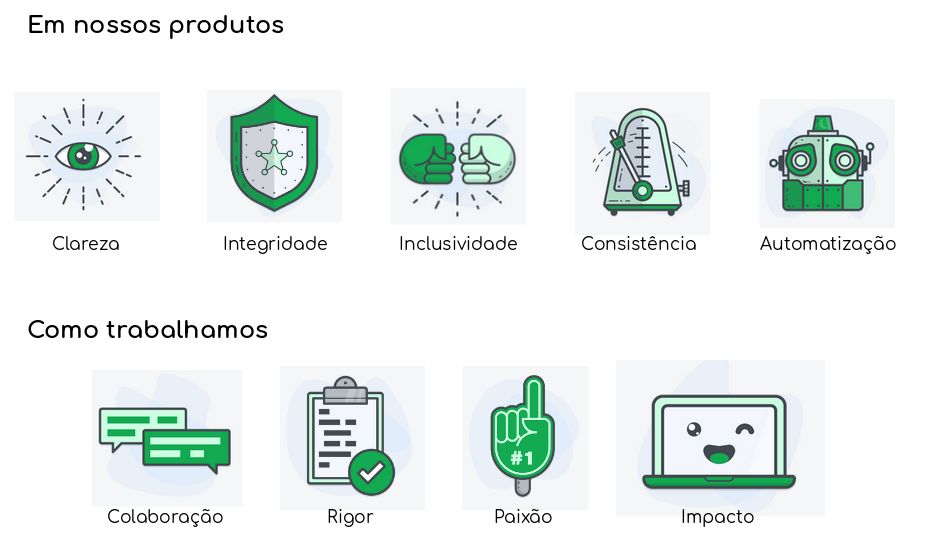
\includegraphics[width=\linewidth]{./04-figuras/02_referencial_teorico/mongodb-design-principles.png}
	\caption{Princípios de design da Mongodb}
  \label{fig:mongodbDesignPrinciples}
\end{figure}

\begin{quadro}[!htb]
	\centering
	\begin{tabular}{|m{2cm}|m{12cm}|} \hline
		
		\multicolumn{1}{|c|}{\bfseries Princípio de Design} & \multicolumn{1}{c|}{\bfseries Descrição} \\\hline
		
		 Clareza & Através do uso de padrões familiares, fluxos de trabalho guiados, instruções em linha e informações contextuais, nossos produtos são compreendidos sem a necessidade de um manual, quando possível, e fornecem acesso fácil à documentação concisa e clara onde necessário. A terminologia é cuidadosamente considerada e mapeia de perto o propósito ou conceito que descreve. \\\hline
		 
		 Integridade & As informações comunicadas ao usuário são precisas e completas. A transparência total instiga confiança na resiliência e segurança do produto, o que é crucial para o gerenciamento de infraestrutura crítica \\\hline
		 
		 Inclusividade & Nossos produtos atendem a todos, desde iniciantes que aprendem a usar o MongoDB pela primeira vez até especialistas da área. Quando um iniciante se sente preso, o produto fornece orientação. Quando um especialista deseja um atalho ou recurso avançado, o produto o fornece exatamente como o usuário esperaria. \\\hline
		 
		 Consistência & Os padrões de informação e interação que aparecem em diferentes lugares são consistentes visualmente e conceitualmente. Isso permite que os usuários movam-se com fluidez através de nossos produtos, confiantes de que o que aprenderem em um deles será transferido para todos os outros. \\\hline
		 
		 Automatização & Nossos produtos transmitem uma compreensão de que as vezes o melhor design é invisível para o usuário. Quando automatizamos uma tarefa, reduzimos a chance de erro do usuário, levando a uma experiência geral mais segura. Nossos produtos automatizam quando possível, deixando o controle com o usuário quando necessário. \\\hline
		 
		 Colaboração & Reconhecemos que o melhor trabalho vem da colaboração diligente. Trabalhamos lado a lado com outros designers, engenheiros e gerentes de produto. \\\hline
		 
		 Rigor & Não estamos satisfeitos com nossas soluções até que as testamos e comprovamos sua eficácia. Nós validamos ideias e conceitos no início do processo de design, antes que  qualquer protótipo seja desenvolvido. Dados é o que nos guia. \\\hline
		 
		 Paixão & Somos intensamente apaixonados pelo nosso trabalho. Nós nos esforçamos para um nível de excelência que encanta o usuário. Mesmo detalhes aparentemente imperceptíveis recebem atenção especial. \\\hline
		 
		 Impacto & Valorizamos o impacto nas nossas entregas. Reconhecemos que nossas ferramentas e processos, enquanto evoluindo e melhorando constantemente, são apenas um meio de alcançar resultados positivos para o usuário. \\\hline
			
	\end{tabular}
	\caption{Princípios de design da Mongodb}
	\label{table:mongodbDesignPrinciples}
\end{quadro}

Já a Pluralsight, atualmente uma das maiores plataformas de cursos online de tecnologia, definiu seus princípios de forma a guiar a maneira como se comunica com seu público alvo. A \autoref{fig:pluralsightDesignPrinciples} detalha tais princípios.

\begin{figure}
	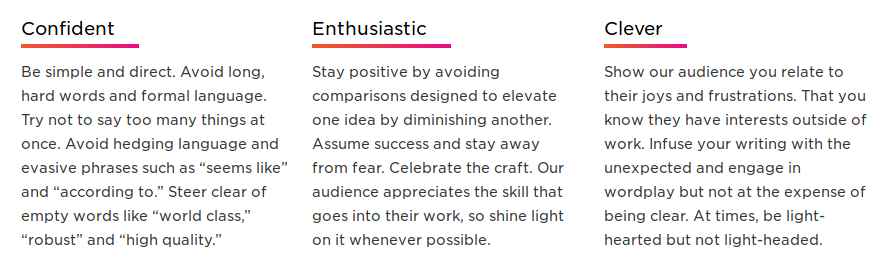
\includegraphics[width=\linewidth]{./04-figuras/02_referencial_teorico/pluralsight-principles.png}
	\caption{Princípios de design da Pluralsight}
	\fonte{Adaptado de \citeonline{pluralsightDesignPrinciples}}
  \label{fig:pluralsightDesignPrinciples}
\end{figure}

Percebe-se, dados os dois exemplos apresentados, que a abordagem adotada pelas empresas na definição dos seus princípios pode variar. Não existe consenso em qual aspecto a organização deve focar. Cada empresa tem seu próprio contexto e cabe a ela aplicar os princípios da melhor maneira possível \cite{kholmatova2017design}.

Princípios de design devem ser relacionáveis uns aos outros, fáceis de se lembrar e limitados em número. Em contrapartida, devem ser específicos o suficiente para serem capazes de auxiliar os designers a tomarem decisões e julgar opções de maneira consistente \cite{kholmatova2017design}.

\subsection{Tom de voz}
\label{subsec:tomVoz}

No domínio verbal, os guias de tom de voz ajudam a definir a maneira com que uma organização se comunica com seu público alvo \cite{ruissalo2018operating}.

De acordo com \citeonline{impactOfVoiceTone}, o tom de voz tem grande impacto na percepção de confiabilidade, amigabilidade e desejo dos usuários em relação aos produtos e serviços de uma empresa. Dado que grandes organizações podem ter vários times internos, um guia de tom de voz é fundamental para dar diretriz aos times, de forma a garantir uma comunicação coesa e consistente entre a empresa e seus clientes. \citeonline{impactOfVoiceTone} categoriza o tom de voz em quatro dimensões: engraçada \textit{vs} séria, casual \textit{vs} formal, insolente \textit{vs} respeitosa, entusiástica \textit{vs} objetiva.

A Firefox, empresa que mantém um navegador para internet como produto, utilizou a categorização proposta por \cite{impactOfVoiceTone}. Como pode ser visto pelas Figuras \ref{fig:firefoxVoiceToneSerious} e \ref{fig:firefoxVoiceTonePlayful}, existem diferenças na maneira como a empresa se comunica com seus usuários dependendo das circunstâncias. Para situações onde ajudar o usuário é prioridade, como em casos de erros, o tom de voz é mais sério. Por outro lado, em situações onde o objetivo é motivar o usuário a tomar alguma ação --- como \textit{onboarding}, sincronização de dados ou \textit{login} --- o tom de voz é mais descontraído, não deixando de ser respeitoso.

\begin{figure}
	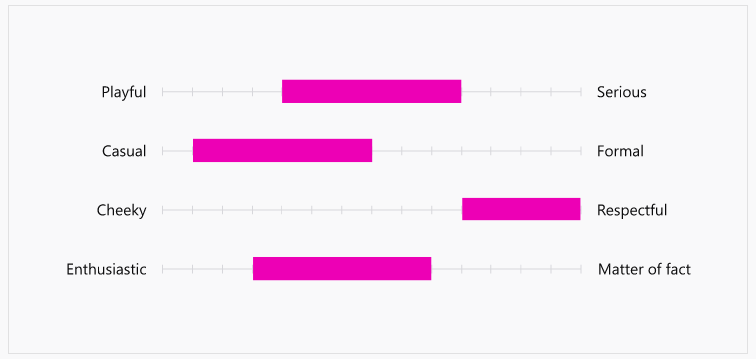
\includegraphics[width=\linewidth]{./04-figuras/02_referencial_teorico/firefox-tone-voice-01.png}
	\caption{Tom de voz para mensagens de suporte críticas da Firefox}
	\fonte{\citeonline{firefoxVoiceTone}}
  \label{fig:firefoxVoiceToneSerious}
\end{figure}

\begin{figure}
	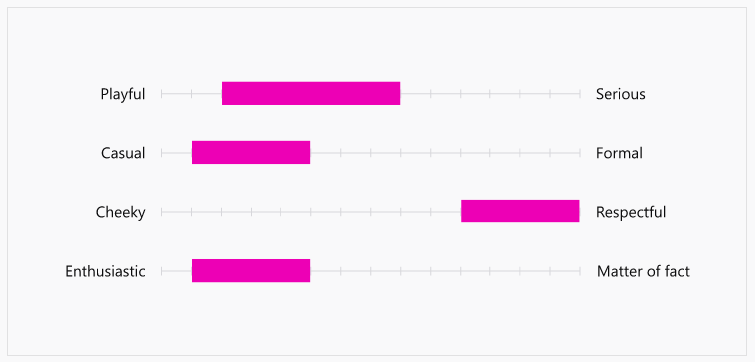
\includegraphics[width=\linewidth]{./04-figuras/02_referencial_teorico/firefox-tone-voice-02.png}
	\caption{Tom de voz para mensagens casuais da Firefox}
	\fonte{\citeonline{firefoxVoiceTone}}
  \label{fig:firefoxVoiceTonePlayful}
\end{figure}

\subsection{Biblioteca de componentes}
\label{sec:bibliotecaComponentes}

Desde a concepção das interfaces de usuário (GUI), a relevância da consistência nas interfaces através dos diferentes produtos de uma organização foi percebida imediatamente \cite{ruissalo2018operating}. Para sanar esse problema, foi proposta a definição das chamadas bibliotecas de componentes. A \autoref{fig:bootstrapStyleGuide} apresenta um exemplo de biblioteca de componentes que é muito utilizada pela indústria: o Bootstrap.

As bibliotecas de componentes tradicionais eram focadas em padronizar o uso dos componentes do produto, como tipografia, imagens e ilustrações, cores, leiaute e outros elementos gráficos \cite{ruissalo2018operating}. Eram, portanto, focadas somente nos aspectos visuais das aplicações, definindo o que era esperado a ser apresentado para o usuário final.

De acordo com \citeonline{taylor2007software}, design no contexto de desenvolvimento de software está mais diretamente ligado na arquitetura dos produtos ao invés de um mero padrão de estilização. Essa é a razão pela qual o design pode, e deve, estar mais próximo da implementação do software. Tal abordagem vai de encontro com um antigo dogma: guias de estilo e bibliotecas de componente são propriedade dos designers \cite{ruissalo2018operating}. Espera-se que as bibliotecas de componentes sejam o resultado do trabalho conjunto de designers e desenvolvedores.

\begin{figure}
	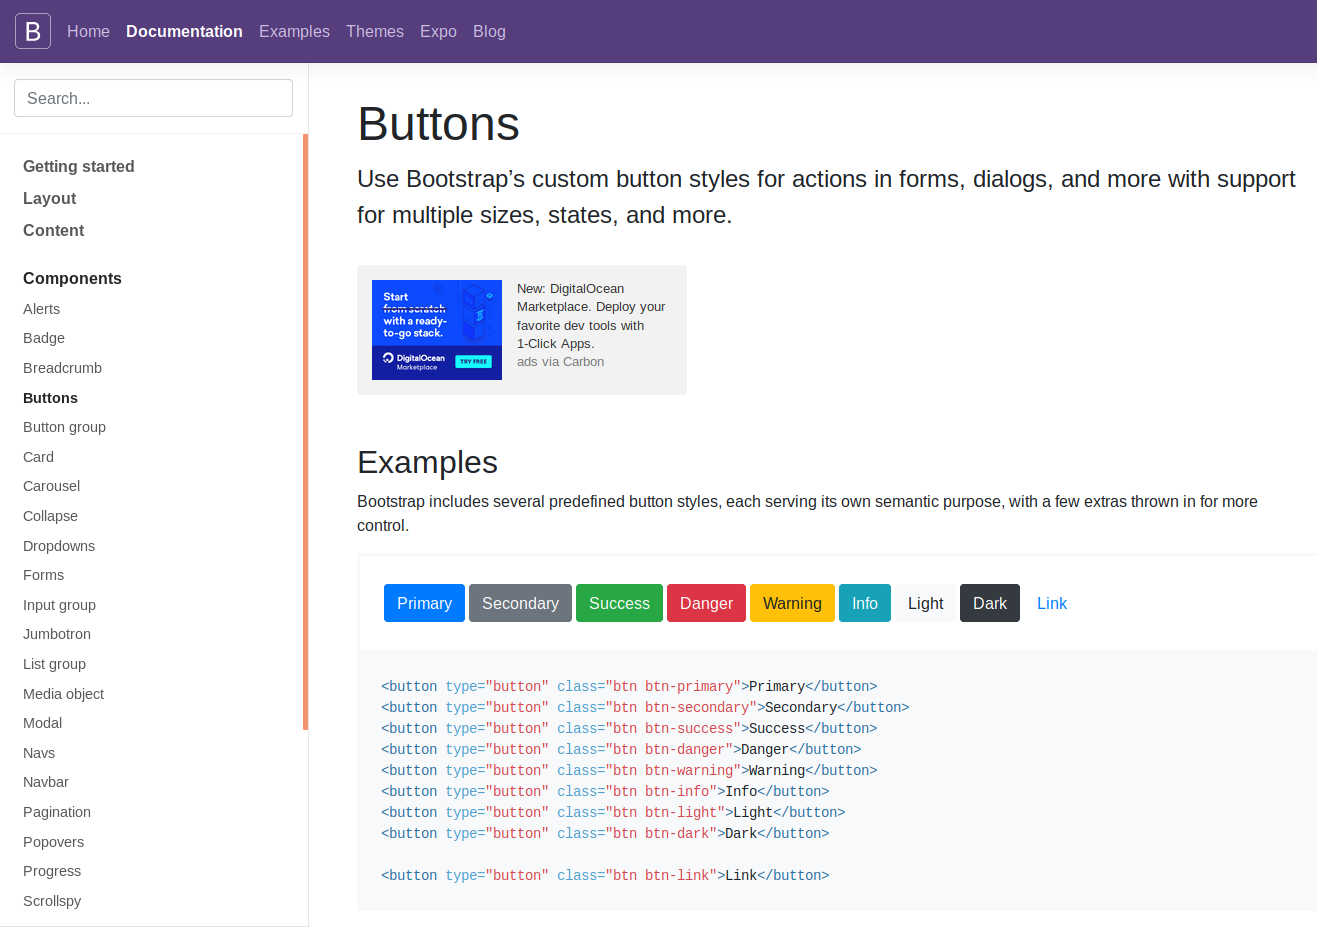
\includegraphics[width=\linewidth]{./04-figuras/02_referencial_teorico/bootstrap.png}
	\caption{Exemplo de biblioteca de componentes}
	\fonte{\citeonline{bootstrapStyleGuide}}
  \label{fig:bootstrapStyleGuide}
\end{figure}

\section{\textit{Atomic Design}}
\label{sec:atomicDesign}

Conforme apresentado na seção anterior, \textit{Design Systems} se propõem a revolucionar a forma como se constroi interfaces de usuário a nível profissional. Entretanto, a forma como são apresentados seus conceitos é, em geral, um tanto quanto subjetiva, ficando a cargo de cada instituição definir a melhor abordagem para o seu problema. Para o caso das bibliotecas de componentes em especial, tanta liberdade assim poderia acarretar em problemas de escalabilidade da solução.

Com o intuito de definir uma metodologia para a implementação técnica de um \textit{Design System}, \citeonline{frostAtomicDesign} buscou na química inspiração para a resolução do problema. A ideia residia no fato de que toda matéria --- seja sólida, líquida, gasosa, simples, complexa, etc --- é composta por unidades minúsculas chamadas átomos. Tais átomos, combinados entre si, formam unidades mais complexas, conhecidas como moléculas. Essas, por sua vez, combinadas formam estruturas ainda mais complexas chamadas organismos. E assim é expressa toda a matéria do universo.

Analogamente à matéria, interfaces de usuários também podem ser expressas por componentes menores. Isso significa que é possível construir interfaces bastante complexas através de um conjunto de componentes menores e mais simples. A \autoref{fig:periodicTable} ilustra e categoriza elementos HTML a níveis atômicos.

\begin{figure}
	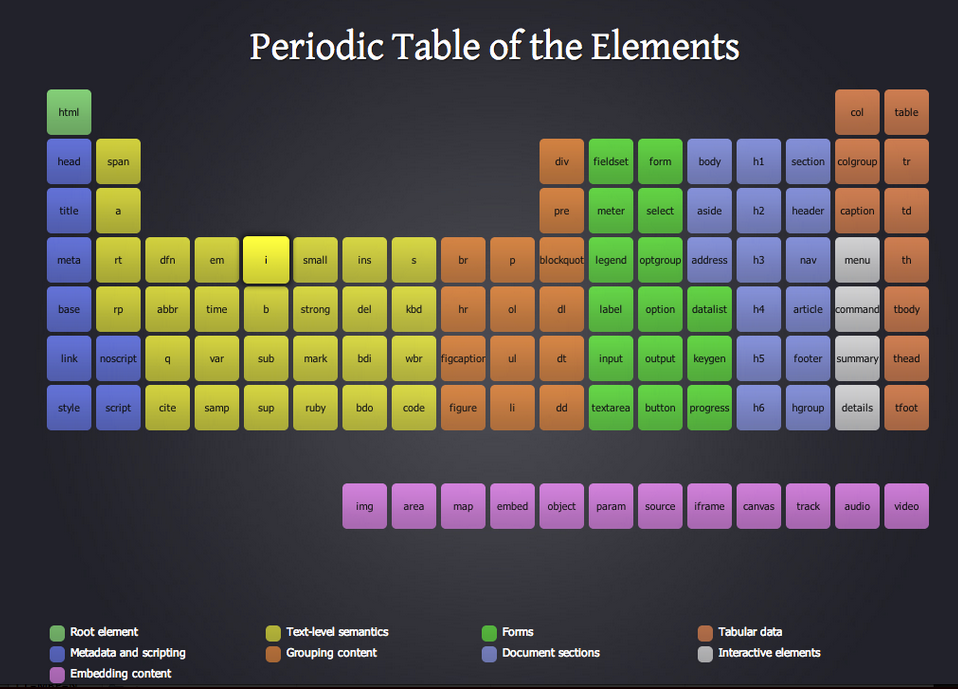
\includegraphics[width=\linewidth]{./04-figuras/02_referencial_teorico/periodic-table.png}
	\caption{Tabela períodica de elementos HTML proposta por Josh Duck}
	\fonte{\citeonline{frostAtomicDesign}}
  \label{fig:periodicTable}
\end{figure}

Dessa forma, \citeonline{frostAtomicDesign} defende a existência de cinco níveis distintos no \textit{Atomic Design}: Átomos, Moléculas, Organismos, Templates e Páginas. A \autoref{fig:atomicDesignLevels} ilustra tais níveis e a forma como eles comunicam entre si.

\begin{figure}
	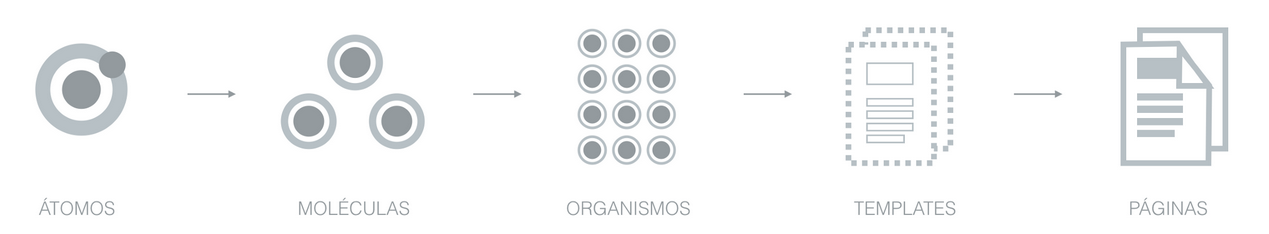
\includegraphics[width=\linewidth]{./04-figuras/02_referencial_teorico/atomic-levels.png}
	\caption{Níveis do \textit{Atomic Design}}
	\fonte{\citeonline{frostAtomicDesign}}
  \label{fig:atomicDesignLevels}
\end{figure}

\subsection{Átomos}
\label{subsec:atomos}

Átomos são os blocos básicos para construção da matéria. Aplicados no universo de interfaces de usuário Web, átomos são as \textit{tags} HTML, como um \textit{input}, botão, \textit{label}, etc.

Assim como os átomos da natureza, eles não são muito úteis de serem manipulados individualmente. Entretanto, cumprem um papel fundamental na construção da biblioteca de componentes, uma vez que todos os componentes mais complexos do sistema são construídos com base neles.

\subsection{Moléculas}
\label{subsec:moleculas}

Tudo começa a ficar mais tangível quando combinamos átomos. As moléculas são um conjunto de átomos distintos que ficam encapsulados juntos. São a espinha dorsal de todo o \textit{Design System}.

Por exemplo, um \textit{label}, um botão e um \textit{input} individualmente não são muito úteis para o usuário final, porém juntos eles formam um formulário que pode de fato gerar valor para o interlocutor.

Construir moléculas a partir de átomos estimula os desenvolvedores a seguir a mentalidade de "faça uma vez, mas faça direito" \cite{frostAtomicDesign}.

\subsection{Organismos}
\label{subsec:organismos}

Organismos são grupos de moléculas que juntas formam uma seção relativamente complexa e distinta da interface de usuário. Examplos de organismos poderiam ser: o cabeçalho de uma página, a seção de menu, etc.

Como organismos já estão em um nível bastante concreto, conseguem definir a estrutura da interface do usuário com bastante clareza. São comumente utilizados como base para uma conversa com clientes finais de um dado produto, uma vez que conseguem transmitir a ideia de valor de uma funcionalidade.

Construir organismos a partir de moléculas estimula os desenvolvedores a construir componentes portáveis e reusáveis \cite{frostAtomicDesign}.

\subsection{Templates}
\label{subsec:templates}

Chegando no nível de templates, abre-se mão da analogia à química para se valorizar uma linguagem que faça mais sentido para os clientes da aplicação. Templates consistem em um conjunto de organismos que compõem uma página. Aqui, começa-se a visualizar o resultado final do design, podendo-se visualizar o leiaute em ação.

A \autoref{fig:atomicDesignTemplate} apresenta um exemplo de um template baseado em \textit{Atomic Design}.

\begin{figure}
	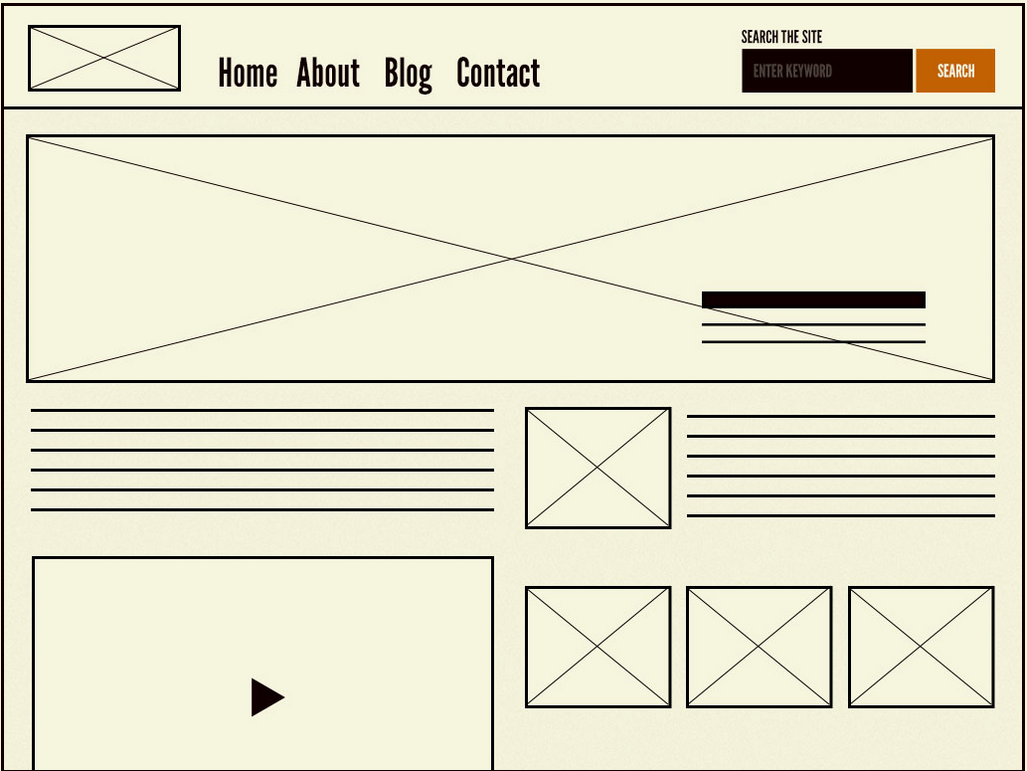
\includegraphics[width=\linewidth]{./04-figuras/02_referencial_teorico/ad-template.png}
	\caption{Exemplo de template}
	\fonte{\citeonline{frostAtomicDesign}}
  \label{fig:atomicDesignTemplate}
\end{figure}

\subsection{Páginas}

Páginas são instâncias específicas de um dado template. Nesse momento, conteúdos de marcação são substituídos por valores reais a serem utilizados na interface de usuário.

Esse estágio é crucial pois é nele onde se testa a efetividade do \textit{design system}. Visualizando todos componentes em um mesmo ambiente facilita o trabalho de validar e eventualmente modificar algum átomo, molécula, organismo ou template, de forma a atingir melhores resultados.
  % Fundamentação teórica
% -----------------------------------------------------------------------------
% Trabalhos Relacionados
% -----------------------------------------------------------------------------

\chapter{Trabalhos Relacionados}
\label{chap:trabRelac}

Neste capítulo são discutidos trabalhos que foram tomados como base para a construção do presente projeto. Levando em consideração que o tema abordado está sendo discutido e aplicado com bastante afinco na indústria de tecnologia, foram selecionados quatro trabalhos para análise, sendo deles um com viés acadêmico e os outros três com viés de mercado. 

A primeira parte do capítulo é focada em apresentar a dissertação de mestrado de Miika Ruissalo, que trata-se de um estudo de viabilidade de implementação de \textit{design system} em uma grande empresa de tecnologia e telecomunicações finlandesa. Em seguida, são apresentados três casos de implementações do \textit{design system} em empresas consolidadas no mercado: Ryte, Gusto e Airbnb. Em cada um dos casos, foram destacadas as motivações e aprendizados adquiridos durante o processo de implementação.

Finaliza-se o capítulo com uma breve discussão a respeito das semelhanças identificadas entre os diferentes trabalhos.

\section{Dissertação de mestrado de Miika Ruissalo}
\label{sec:teseMestrado}

Ao se investigar a ocorrência de trabalhos relacionados na literatura, aquele que apresentou maior similidaridade, no que se diz respeito ao seu propósito, foi a dissertação de mestrado de \citeonline{ruissalo2018operating}.

Entitulada \textit{Operating a design system in a large software company}, \citeonline{ruissalo2018operating} discute o fenômeno \textit{design system} como proposta de solução para problemas de consistência e escalabilidade que empresas de tecnologia acabam vivenciando durante o fluxo de desenvolvimento de seus produtos em larga escala. A fase empírica do projeto se demonstrou como um estudo da aplicação da metodologia por uma grande empresa de tecnologia e telecomunicações finlandesa. A empresa em questão havia passado por um processo de restruturação do seu design, criando seu próprio \textit{design system}. Tal evento ocorreu três anos antes do desenvolvimento da dissertação.

O experimento teve duração de seis meses, período ao qual foram observados sete dos vários times de desenvolvimento de produtos da empresa. O grupo amostral escolhido para o experimento foi cuidadosamente selecionado para garantir que todos os contextos chave da organização seriam cobertos pela pesquisa. O \autoref{table:ruissaloTeams} apresenta as características de cada um dos times selecionados.

\begin{quadro}
  \centering
  \begin{tabular}{|m{2cm}|m{4cm}|m{8cm}|} \hline
    
    \multicolumn{1}{|c|}{\bfseries Time} & \multicolumn{1}{c|}{\bfseries Contexto e Plataforma} & \multicolumn{1}{c|}{\bfseries Considerações importante} \\\hline
    
     Time 1 & B2B - Web & Um designer do time criou parte considerável dos \textit{assets} do sistema \\\hline
     
     Time 2 & Mercado consumidor - Web e Mobile & Começou a utilizar tecnologias relevantes recentemente, incluindo o \textit{design system} \\\hline
     
     Time 3 & Mercado consumidor - Web & Um dos três times que construiu a base de toda a plataforma \\\hline
     
     Time 4 & Ferramenta B2B - Web & Time surgiu pouco tempo antes da realização do experimento \\\hline
     
     Time 5 & Ferramenta B2B - Mobile & A criação do \textit{design system} não levou em consideração o contexto desse time \\\hline
     
     Time 6 & Mercado consumidor - Web & Trabalha com projetos de curta duração e que geram impacto rapidamente \\\hline
     
     Time 7 & Mercado consumidor - Plataforma específica & Não pode utilizar o \textit{design system} devido ao contexto da plataforma específica não o permitir \\\hline
     
      
  \end{tabular}
  \caption{Característica dos times estudados por \citeonline{ruissalo2018operating}}
  \fonte{\citeonline{ruissalo2018operating}}
  \label{table:ruissaloTeams}
\end{quadro}

A metodologia adotada pela dissertação consistiu basicamente em duas grandes fases: observação e entrevistas. Na primeira fase, \citeonline{ruissalo2018operating} dedicou seu tempo à observar o dia-a-dia de cada um dos times selecionados, estando posicionado estratégicamente próximo de três destes. Na segunda fase, o pesquisador realizou entrevistas com dois grupos distintos de profissionais: designers e desenvolvedores. Cada grupo, portanto, experimentou um roteiro de entrevista diferente do outro.

Como resultado do experimento, foi observado que uma das maiores dores dos profissionais de desenvolvimento de produto é a falta de uma fonte única da verdade. Esse foi um dos principais argumentos utilizado pelos times quando a empresa sob estudo optou por desenvolver seu \textit{design system}. A maioria dos benefícios apontados no \autoref{chap:fundamentacaoTeorica} do presente trabalho foi parceptível na empresa finlandesa, tanto na visão da organização quanto na visão dos designers e desenvolvedores. Consistência, poder de reusabilidade e velocidade no desenvolvimento foram características observadas no produto e nos times analisados pela dissertação, exemplificando assim a metodologia de \textit{design system} como um verdadeiro sucesso no desenvolvimento de produtos digitais em uma grande organização.

\section{Ryte}
\label{sec:ryte}

A Ryte é uma organização cujo produto principal oferece a capacidade de monitoramento, análise e otimização dos \textit{sites} de seus clientes de forma a garantir melhores taxas de desempenho. Ela conta atualmente com uma cartela de mais de 500.000 usuários ativos em sua plataforma.

Seu produto surgiu como resultado de uma repaginação do antigo \textit{OnPage.org}. No artigo \textit{Lessons learned building a Design System for 500,000+ users at Ryte} \cite{ryteDesignSystem}, o autor discute os desafios que surgiram como consequência dessa transição.

O artigo tem início com \citeonline{ryteDesignSystem} afirmando que, nos momentos iniciais da transição, toda a equipe estava bastante motivada. Por esse motivo, a plataforma ganhou forma com bastante velocidade, porém sem consistência alguma. Os diversos times que compunham a organização trabalhavam isoladamente uns dos outros, produzindo assim diferentes soluções para um mesmo problema. Com quatro meses de projeto, percebeu-se que o caminho que estava sendo traçado não era sustentável e que medidas deveriam ser tomadas imediatamente.

Naquele momento, a empresa enfrentava três grandes problemas que deveriam ser solucionados o quanto antes.

O primeiro deles era o fato de que todos os produtos da plataforma eram muito diferentes uns dos outros, tanto visualmente quanto em relação à experiência do usuário ao utilizá-los. Com 11 tipos distintos de \textit{pop-ups}, 23 tipos de botões e 67 tons de cinza diferentes, os usuários acabavam tendo que reaprender os mesmos conceitos quando utilizavam uma nova ferramenta disponibilizada pela plataforma.

O segundo problema era um pouco mais grave: um processo de design lento e ineficiente. O tempo para se construir novas funcionalidades era elevado, uma vez que era preciso reconstruir a grande maioria dos componentes presentes na entrega do zero.

Por fim, o último ponto a ser resolvido era a falta de identidade de marca no mercado. Além de inconsistências na plataforma, não havia co-relação alguma entre os mecanismos de marketing e a plataforma em si.

Inspirada em empresas como Shopify, Atlassian e Hubspot, a Ryte buscou na metodologia do \textit{design system} uma solução para os seus problemas. A abordagem utilizada consistia basicamente em dois componentes: um arquivo Sketch e um repositório Git compartilhados. Percebe-se que não foram abordados fatores como tom de voz e princípios de design nessa primeira versão. Além disso, não existe interligação clara entre artefatos de design e artefatos de desenvolvimento e a justificativa para tal decisão reside no fato de que o time identificou problemas de escalabilidade ao se unir os dois mundos.

Como resultado imediato da implementação do \textit{design system} percebeu-se: processo de design oito vezes mais rápido, mais velocidade no desenvolvimento de novas funcionalidades e um maior poder de escalabilidade. \citeonline{ryteDesignSystem} ainda compartilha no artigo alguns dos aprendizados que o time vivenciou ao longo do processo. Tais aprendizados são consolidados e apresentados no \autoref{table:ryteLessonsLearned}.

\begin{quadro}
  \centering
  \begin{tabular}{|m{4cm}|m{10cm}|} \hline
    
    \multicolumn{1}{|c|}{\bfseries Aprendizado} & \multicolumn{1}{c|}{\bfseries Comentário} \\\hline
    
     Não reinventar a roda & Existem várias bibliotecas de componentes prontas no mercado que podem ser utilizadas como base. \\\hline
     
     A biblioteca de componentes é um documento vivo & Ao se desenvolver novas funcionalidades, constantemente surgem novos componentes a serem incluidos na biblioteca. Deve-se evitar ao máximo incluir novos componentes semelhantes a algum já existente. Nesses casos, é preferível dar manutenção a este. \\\hline
     
     Aproximar o produto dos mecanismos de marketing & Podem existir problemas durante essa unificação -- como diferentes tamanhos de fonte, por exemplo --, porém isso é necessário. \\\hline
     
     Envolver pessoas chave no processo & Certificar-se de que existem pessoas com um bom \textit{background} técnico para a tomada de decisões importantes. Também é importante envolver pessoas com diferentes contextos no processo. \\\hline
     
     Comunicação com o desenvolvedor é fundamental & Transmitir a importância do \textit{design system} para o desenvolvedor é fundamental, pois só assim haverá a garantia de que as decisões tomadas pela metodologia serão refletidas no produto. \\\hline
      
  \end{tabular}
  \caption{Aprendizados da implementação do \textit{design system} da Ryte.}
  \fonte{\citeonline{ryteDesignSystem}}
  \label{table:ryteLessonsLearned}
\end{quadro}

\section{Gusto}
\label{sec:gusto}

A Gusto é uma empresa que facilita o gerenciamento de folhas de pagamento e benefícios dos funcionários de seus clientes. Fundada em 2011, atualmente conta com cerca de 60.000 clientes ativos em sua plataforma.

Foi iniciado, em 2016, um projeto de criação de um \textit{design system} para a organização. No artigo \textit{Design Systems at Gusto: Part I}, escrito por Robin Rendle \cite{gustoDesignSystem}, é apresentado todo o processo de desenvolvimento do mesmo.

Problemas nos processos de design e desenvolvimento eram as principais motivações para a criação do \textit{design system}. Na época, o time de produto da empresa era composto por nove designers de produto e muitos engenheiros de desenvolvimento. Gerir uma comunicação eficaz entre os diferentes times e profissionais envolvidos na plataforma era um grande desafio que, até então, não havia sido solucionado. Não existia, ainda, nenhuma biblioteca de componentes que guiasse a tomada de decisão de design dos times. Como consequência, a base de código-fonte \textit{frontend} da plataforma se tornou muito grande e confusa, o que impactava diretamente a capacidade de escalabilidade do produto.

Foi nesse momento que Rendle decidiu, de maneira proativa, iniciar os trabalhos de construção do novo \textit{design system} da Gusto. Durante esse processo foram acumulados alguns aprendizados, que foram consolidados no \autoref{table:gustoLessonsLearned}.

\begin{quadro}
\centering
\begin{tabular}{|m{4cm}|m{10cm}|} \hline
	
	\multicolumn{1}{|c|}{\bfseries Aprendizado} & \multicolumn{1}{c|}{\bfseries Comentário} \\\hline
	
	 É impossível construir um \textit{design system} sozinho & A pior coisa que se pode fazer para uma empresa é se provar como sendo o seu colaborador mais inteligente. Esse tipo de postura gera desconforto por parte dos outros membros da empresa e negligencia pontos de vista diferentes do seu. \\\hline
	 
	 Um \textit{design system} não precisa estar completo para ser útil & Como seu propósito é sanar os problemas de toda uma organização, a nível de design de produto, é comum se empregar muito esforço para a construção de um \textit{design system} perfeito. A verdade é que, por mais simples que ele seja, um \textit{design system} por si só já gera um valor muito grande, uma vez que ele centraliza as tomadas de decisões de design de produto da empresa. \\\hline
	 
	 \textit{Design Systems} surgem e morrem por conta de sua documentação & A documentação de um componente é tão importante quanto o componente em si. Caso a maneira como um componente deve ser manipulado não seja auto-explicativa, seus usuários tenderão a evita-lo. \\\hline
	 
	 Um \textit{design system} é um repositório de conhecimento & \textit{Design Systems} não são importantes somente por representar precisamente a base de código, mas também por diminuir a complexidade social de uma organização, estimulando a comunicação e concentrando o conhecimento. \\\hline
    
\end{tabular}
\caption{Aprendizados da implementação do \textit{design system} da Gusto}
\fonte{\citeonline{gustoDesignSystem}}
\label{table:gustoLessonsLearned}
\end{quadro}

Rendle finaliza seu artigo destacando uma das vantagens de se implementar um \textit{design system}: garantir que a comunicação entre todos os membros envolvidos no produto ocorra de maneira fluida e de acordo com as diretrizes de design e produto da organização. Na \autoref{fig:socialComplexityIncrease}, o autor ilustra a maneira como a complexidade de comunicação dentro de uma empresa aumenta consideravelmente conforme novos talentos são incluídos no processo. Reintara, ainda, o papel fundamental de um \textit{design system} como facilitador da comunicação entre os times.

\begin{figure}
	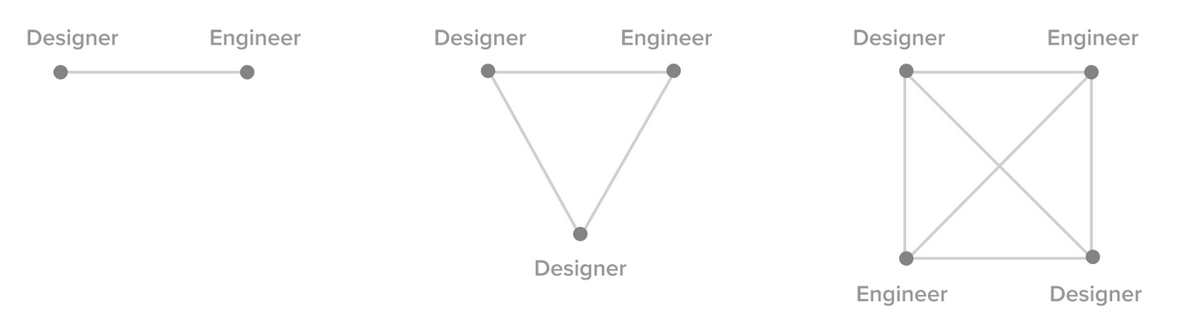
\includegraphics[width=\linewidth]{./04-figuras/03_trabalhos_relacionados/social-complexity.png}
    \caption{Evolução da complexidade social de uma empresa}
    \fonte{\citeonline{gustoDesignSystem}}
    \label{fig:socialComplexityIncrease}
\end{figure}

\section{Airbnb}
\label{sec:airbnb}

Como último exemplo de trabalho relacionado ao presente documento, será apresentado o estudo de caso de implementação do \textit{design system} da Airbnb. Com sede em San Francisco - California, Estados Unidos, a Airbnb é uma famosa empresa que opera um mercado on-line global de serviços de hospedagem acessível através de seu site e aplicativo para dispositivos móveis.

No artigo \textit{Building a Visual Language}, produzido por Karri Saarinen e disponibilizado diretamente no site oficial da empresa, discorre-se sobre a trajetória de criação do sistema, poderando-se suas motivações e aprendizados adquiridos ao longo do processo.

Devido ao seu crescimento acelerado, problemas de escalabilidade do produto surgiram rapidamente, conforme a empresa conquistava maiores parcelas do seu mercado e aumentava o tamanho de sua equipe de desenvolvimento.

O primeiro problema apresentado foi a falta de padrões disseminados entre as equipes. Esse fator contribuia para a criação de uma variedade de artefatos que resolvem o mesmo problema, muitas vezes ocasionando em experiências de usuários distintas ao longo de toda a plataforma.

Em seguida, o artigo menciona o problema de se ter múltiplos designers e \textit{stakeholders} trabalhando em uma mesma plataforma. A maior dificuldade, nesse ponto, seria manter consistência em todo o produto.

Outro fator motivador para a criação do \textit{design system} foi a necessidade de se dar suporte a múltiplas plataformas e dispositivos. Sem uma biblioteca de componentes flexível, o fenômeno do retrabalho acaba sendo inevitável. Uma mesma funcionalidade deveria ser implementada várias vezes, dependendo da quantidade de plataformas que a empresa suportasse.

Para sanar os problemas citados, a Airbnb decidiu por construir o seu próprio \textit{design system}. O processo de criação foi exaustivo, porém o resultado final foi um sucesso. Dos exemplos citados no presente trabalho, o \textit{design system} da Airbnb é, sem dúvidas, o mais completo. Nele, além da biblioteca de componentes, também foram trabalhados os artefatos de princípios de design e tom de voz. Por isso, o trabalho realizado pela Airbnb é hoje uma das referências do mercado no que se diz respeito a \textit{design systems}.

Saarinen também compartilha alguns dos aprendizados adquiridos pela sua equipe no artigo. Tais aprendizados foram consolidados no \autoref{table:airbnbLessonsLearned}.

\begin{quadro}
\centering
\begin{tabular}{|m{4cm}|m{10cm}|} \hline

	\multicolumn{1}{|c|}{\bfseries Aprendizado} & \multicolumn{1}{c|}{\bfseries Comentário} \\\hline
	
	 Nem todos os componentes são criados igualmente & Alguns componentes podem ter variações de implementações para diferentes plataformas. Em alguns casos, manter esse segregação é mais saudável e facilita a manutenção. \\\hline
	 
	 Documentação & A atividade de documentação dos componentes deve fazer parte do processo de criação, independentemente dos prazos de entrega. A falta de documentação dos componentes pode gerar muita confusão. \\\hline
    
\end{tabular}
\caption{Aprendizados da implementação do \textit{design system} da Airbnb}
\fonte{\cite{airbnbDesignSystem}}
\label{table:airbnbLessonsLearned}
\end{quadro}

Pode-se perceber, principalmente pelos depoimentos apresentados nas Seções \ref{sec:ryte}, \ref{sec:gusto} e \ref{sec:airbnb}, que as motivações que levam empresas a adotarem o \textit{design system} internamente são muito semelhantes. A dificuldade de se manter consistência no produto, a baixa velocidade de desenvolvimento e a falta de um repositório único que concentre as decisões de design são problemas comuns em empresas de tecnologia. Nesse contexto, o \textit{design system} vem se mostrando uma solução bastante eficaz.

No capítulo seguinte é apresentada a metodologia empregada pelo presente projeto para validar a eficácia de se utilizar um \textit{design system}, sob o ponto de vista de um desenvolvedor.
 % Trabalhos relacionados
% -----------------------------------------------------------------------------
% Metodologia
% -----------------------------------------------------------------------------

\chapter{Metodologia}
\label{chap:metodologia}

O desenvolvimento do presente trabalho parte da premissa de que designers e desenvolvedores não tem uma linguagem comum durante a execução de suas atividades, produzindo artefatos isoladamente uns dos outros. Por conta disso, problemas como inconsistência no produto, baixa velocidade de desenvolvimento de novas interfaces de usuário e dificuldade em se dar manutenção em interfaces já existente, são alguns dos fatores que comprometem a capacidade de escalabilidade dos produtos de empresas de tecnologia.

Para entender se a proposta de metodologia de um \textit{design system} é eficiente para resolver tais problemas no processo de design e desenvolvimento \textit{frontend} das organizações, o autor deste trabalho tomou como cobaia para um experimento uma empresa de tecnologia: Dito. Com 11 anos de história, a Dito é uma \textit{startup} mineira que vem passando por um processo de crescimento bastante acelerado. Por conta disso, muitos dos sintomas que impedem a escalabilidade do seu produto já são perceptíveis internamente na organização. 

O experimento realizado tem como objetivo construir um protótipo de um \textit{design system}, validando se os benefícios indicados pela teória da metodologia realmente se manifestam na prática. Sabendo que a construção de um \textit{design system} do zero é uma tarefa muito complexa, o autor optou por incluir somente o artefato de biblioteca de componentes no protótipo. Como temática para o projeto, foi proposta a construção de um sistema de gestão de funcionários da empresa, intitulado \textit{DitoFeras}.

A metodologia adotada no desenvolvimento deste trabalho é dividida em 5 grandes estágios, ilustrados através da \autoref{fig:metodology}.

\begin{figure}
	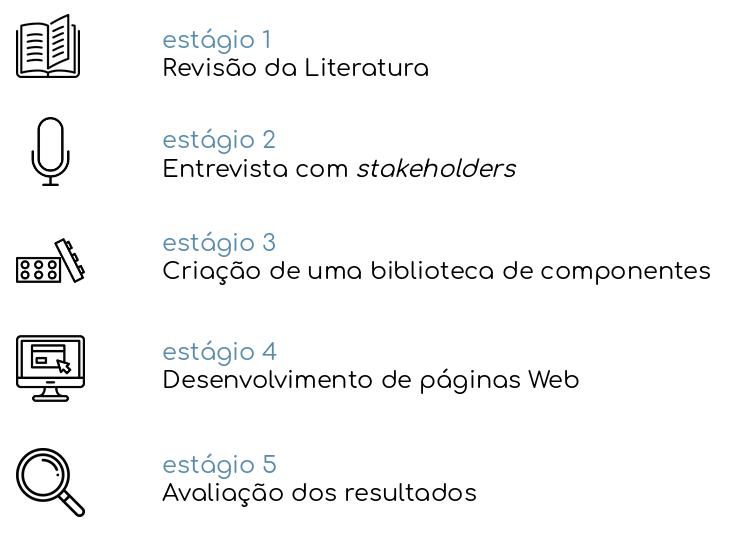
\includegraphics[width=\linewidth]{./04-figuras/04_metodologia/metodologia.png}
  \caption{Esquema da metodologia}
  \fonte{Próprio autor}
  \label{fig:metodology}
\end{figure}

O estágio inicial da metodologia tinha como objetivo realizar uma revisão de trabalhos e estudos relacionados a \textit{design systems}, tanto no âmbito acadêmico quanto no industrial. As informações adquiridas nesse estágio foram apresentadas mais detalhadamente nos capítulos \ref{chap:fundamentacaoTeorica} e \ref{chap:trabRelac} deste trabalho e serviram como base de conhecimento para os estágios seguintes.

No segundo estágio, foram realizadas entrevistas com os principais \textit{stakeholders} do projeto: designers e desenvolvedores. A idéia das entrevistas é validar se os mesmo se sentem incomodados com a maneira que os processos de design e desenvolvimento da empresa são adotados atualmente. Em caso positivo, seguiria-se para o estágio seguinte da metodologia.

No estágio 3, caso seja comprovada sua necessidade pelo estágio anterior, daria-se início ao desenvolvimento de uma biblioteca de componentes simples. Seguindo a idéia da Ryte \cite{ryteDesignSystem} para a criação do seu \textit{design system}, a versão de protótipo da biblioteca de componentes da Dito seria baseada em 2 artefatos: um guia de design, construído utilizando a ferramenta Figma, e um repositório Git com a implementação dos componentes. Com os componentes construídos, seguiria-se para o estágio 4 da metodologia.

O quarto estágio seria aquele que, tomando como base os componentes criados no estágio anterior, construiria algumas páginas Web propostas para o projeto \textit{DitoFeras}. Esperava-se que nessa fase, a velocidade de desenvolvimento das páginas fosse mais rápida do que aquela habitual. Por fim, o último estágio seria aquele que defiriria e mediria as métricas performance do experimento, comprovando ou não a eficácia de um \textit{design system}.

No capítulo seguinte será apresentado detalhadamente os resultados obtidos no segundo estágio da metodologia deste projeto: entrevistas com \textit{stakeholders}.
            % Metodologia
% -----------------------------------------------------------------------------
% Entrevistas com Stakeholders
% -----------------------------------------------------------------------------

\chapter{Entrevistas com \textit{Stakeholders}}
\label{chap:entrevistas}


Como forma de validar a real necessidade de criação de um \textit{design system} na empresa avaliada pelo experimento, foram realizadas entrevistas com os principais \textit{stakeholders} do projeto: designers e desenvolvedores \textit{frontend}. Neste capítulo são apresentados, de maneira consolidada, os resultados obtidos como consequência de tais entrevistas.

Para garantir que os resultados não ficassem restritos em um único contexto da organização, foram selecionados três profissionais, com desafios destintos dentro da empresa, como representantes de cada um dos grupos.

Todas as entrevistas foram gravadas, conforme consentimento dos participantes. Para garantir o anônimato dos envolvidos, todos os dados apresentados neste capítulo estarão associados a nomes de marcação, não expondo nomes e dados pessoais reais dos voluntários.

\section{Designers}
\label{sec:entrevistasDesigners}

De acordo com o roteiro de entrevista ilustrado no Anexo \ref{chap:anexoA} deste projeto, os designers avaliados foram submetidos a algumas perguntas genéricas onde puderam expor um pouco dos detalhes do seu dia-a-dia de trabalho. O \autoref{table:designersResearch} apresenta as características de cada um dos profissionais entrevistados.

\begin{quadro}
\centering
\begin{tabular}{|m{4cm}|m{10cm}|} \hline
	
	\multicolumn{1}{|c|}{\bfseries Voluntário} & \multicolumn{1}{c|}{\bfseries Contexto} \\\hline
	
	 Designer 1 & Profissional mais experiente do grupo, sendo a principal referência de design em toda a organização. Está diretamente envolvido em um projeto mais novo e bastante promissor da empresa, entitulado \textit{DitoPDV}. Nesse projeto, teve a liberdade de definir novos padrões de design que hoje são tomados como referência para todos os novos produtos da empresa. \\\hline
	 
	 Designer 2 & Pilar de design do maior \textit{squad} da empresa, que tem como objetivo dar manutenção e evoluir todo o fluxo de comunicação da plataforma. Está diretamente envolvido com sistemas legados do produto, e tem como principal desafio garantir uma boa experiência do usuário ao longo do uso da plataforma. \\\hline
	 
	 Designer 3 &  Responsável pelo design da área de marketing da organização, estando diretamente envolvido em campanhas de eventos, contratação e lançamento de novos produtos. Também é responsável pelas artes do site e do blog de tecnologia da empresa. \\\hline
    
\end{tabular}
\caption{Características dos designers entrevistados}
\fonte{Próprio autor}
\label{table:designersResearch}
\end{quadro}

A seguir, são apresentados os resultados consolidados de perguntas chave realizadas nas entrevistas.

\textbf{Questão 1:} Contextualize, brevemente, a maneira como os processos de design são adotados na empresa, atualmente.

\begin{quote}
    A maioria das empresas de tecnologia é focada no desenvolvedor. Por isso, grande parte dos processos de desenvolvimento existentes está associada ao código-fonte, sendo o design muitas vezes negligenciado. Por muito tempo essa foi a realidade da Dito, porém nos últimos dois anos a área de design começou a conquistar seu espaço na organização, tendo, pela primeira vez, profissionais especializados da área designados a evoluírem a plataforma com foco no usuário final do produto.
    
    Foi a partir desse momento que iniciaram-se trabalhos para definir os primeiros processos de design da empresa. O primeiro deles foi a inclusão de ferramentas como Sketch e Zeplin \footnote{O Zeplin é uma ferramenta gráfica destinada ao compartilhamento de artes de design em um formato técnico para desenvolvedores \textit{frontend}. Está disponível em <https://zeplin.io>} na rotina dos designers e desenvolvedores \textit{frontend}. Com elas, o designer exerce seu papel de pensar na melhor interface de usuário possível para um dado problema e, após sua prototipação, o desenvolvedor tem acesso a arte de maneira detalhada tecnicamente. Isso fez com que as novas interfaces desenvolvidas, desde então, fossem mais fidedignas àquilo idealizado pelo designer.
    
    Apesar do considerável avanço, ainda entende-se que a empresa está "engatinhando" no que se diz respeito a processos de design. Ainda existe uma visão geral de que design se restringe unicamente à criação de interfaces. No que se tange a concepção de produtos, não está bem definido um processo de design escalável. Pensando nisso, um dos \textit{squads} da empresa vem tentando implacar um novo modelo conhecido como \textit{Double Diamond Design}, proposto pela metodologia de \textit{design thinking}. Tal processo é dividido em fases de imersão, ideação, prototipação e testes de usabilidade, objetivando a construção de produtos de maneira mais rápida e aderente às necessidades do usuários final.
    
    Na área de marketing, por sua vez, o contexto é um pouco diferente: contando apenas com dois profissionais alocadas para gerenciar toda a área, a criação de uma \textit{styleguide} se tornou uma necessidade latente. A maneira encontrada para se ganhar velocidade, e atender à toda a demanda da empresa, foi a criação de templates. Tal \textit{styleguide} \footnote{Sinônimo de guia de estilos e biblioteca de componentes.} foi criada a partir de um dos produtos da plataforma, porém não existe ligação alguma entre os dois artefatos.
\end{quote}

\textbf{Questão 2:} Quais as maiores dificuldades e frustrações que você encontra no seu trabalho, como consequência dos processos atuais de design?

\begin{quote}
    Tendo em vista que a maturidade em design da Dito está passando por um processo de evolução, os designers da empresa ainda precisam empregar uma quantidade de esforço significativa para a construção de novos protótipos de interfaces de usuários, uma vez que a capacidade de reusabilidade de componentes ainda está aquém do ideal. 
    
    Por conta disso, as maiores frustrações do time, em geral, estão relacionadas à impossibilidade de se ter um contato mais próximo com o usuário final do produto. Deseja-se que tarefas de teste de usabilidade e metrificação de maturidade façam parte do processo de design da Dito, porém atualmente isso é inviável pois os designers estão muito ocupados em dar vazão à demandas de criação de novas interfaces.
    
    Também destaca-se a falta de uma figura exclusivamente responsável por definir e garantir que as diretrizes de design estão sendo seguidas pela organização como um todo. Espera-se que essa pessoa também exerça o papel de tutor de talentos menos experientes, papel este inexistente na conjuntura atual da empresa.
\end{quote}

\textbf{Questão 3:} Como são tomadas decisões de design na empresa? E no seu time? Quem são as pessoas envolvidas?

\begin{quote}
    Basicamente, a partir da apresentação de um dado desafio, inicia-se uma fase de análise aprofundada do problema. Durante essa fase, é bastante comum o envolvimento de profissionais de negócio e desenvolvedores para a validação da viabilidade de possíveis soluções. Vez ou outra acontecem alterações nas decisões de design pré-estabelecidas devido à inviabilidade técnica da proposta. Portanto, esse tipo de tomada de decisão já é fruto de um trabalho colaborativo entre diferentes perfis de profissionais.
    
    Entretanto, o núcleo das discussões normalmente acontece no contexto individual do \textit{squad} responsável pelo problema. Não existe consenso geral de diretrizes a serem seguidas pelos times. Dessa forma, o cenário atual é caracterizado pelo trabalho isolado dos designers da empresa. Cada um deles se mantém focado exclusivamente nos desafios do seu próprio \textit{squad}, não sendo comum um intercâmbio de experiências entre os membros da área de design como um todo.
    
    Foram levantadas, ainda, situações em que decisões de design foram tomadas por profissionais de negócio, mesmo quando em desacordo do ponto de vista do designer responsável pela entrega. Devido à falta de autoridade da área, sendo um claro reflexo da imaturidade da mesma, a experiência do usuário acaba sendo prejudicada em detrimento do cumprimento de prazos estabelecidos para entregas.
\end{quote}

\textbf{Questão 4:} Como você classifica a velocidade de desenvolvimento de novas interfaces de usuários atualmente? Por que?

\begin{quote}
    De maneira geral, está mais rápida do que o observado em momentos anteriores à definição dos processos inicias de design, porém poderia estar melhor caso existisse uma biblioteca de componentes bem estruturada.
\end{quote}

\textbf{Questão 5:} Você acredita que um \textit{design system} poderia ser uma opção plausível para alavancar a capacidade de escalabilidade do produto da empresa?

\begin{quote}
    De maneira unânime, sim.

    A padronização de ferramentas e processos é, sem dúvidas, um excelente promotor do potencial de escalabilidade do produto. Estima-se que, com uma biblioteca de componentes bem estruturada, tarefas de prototipação seriam executadas 4 vezes mais rapidamente.
    
    Entende-se, entretanto, que a criação de um \textit{design system} é um projeto bastante ambicioso e complexo, fazendo-se necessário o envolvimento, preferencialmente exclusivo, de uma série de profissionais com nível avançado de senioridade. O resultado final do projeto é um artefato que tem a pretenção de resolver problemas de comunicação de toda uma organização, portanto sua concepção deve ser embasada nas dores de todos os grupos que compõem a empresa.
    
    Ressalta-se ainda que, o processo de criação de um \textit{design system} deve ser encarado como um produto e não um projeto. Para tanto, o mesmo deve estar em constante evolução, mantendo sua documentação viva e atualizada.
\end{quote}

\section{Desenvolvedores \textit{frontend}}
\label{sec:entrevistasDevs}

De acordo com o roteiro de entrevista ilustrado no Anexo \ref{chap:anexoB} deste projeto, os desenvolvedores avaliados foram submetidos a algumas perguntas genéricas onde puderam expor um pouco dos detalhes do seu dia-a-dia de trabalho. O \autoref{table:devsResearch} apresenta as características de cada um dos profissionais entrevistados.

\begin{quadro}
\centering
\begin{tabular}{|m{4cm}|m{10cm}|} \hline
	
	\multicolumn{1}{|c|}{\bfseries Voluntário} & \multicolumn{1}{c|}{\bfseries Contexto} \\\hline
	
	 Desenvolvedor 1 & Profissional que teve mais contato com a base de código-fonte da plataforma. Com mais de 4 anos de colaboração com o produto, teve a oportunidade de participar de vários projetos da empresa. Atualmente, assume o desafio de liderança do \textit{squad} de suporte técnico da organização. \\\hline
	 
	 Desenvolvedor 2 & Principal desenvolvedor do \textit{squad} responsável por manter um dos mais recentes e promissores produtos da empresa. Nesse projeto, teve a oportunidade de trabalhar com tecnologias mais inovadoras do que aquelas utilizadas na base de código-fonte legada da plataforma. \\\hline
	 
	 Desenvolvedor 3 & Mais novo colaborador do \textit{squad} de comunicação da empresa. Está a cerca de 2 meses assumindo o desafio de manter e evoluir sistemas legados de \textit{fronted} da plataforma. \\\hline
    
\end{tabular}
\caption{Características dos desenvolvedores entrevistados}
\fonte{Próprio autor}
\label{table:devsResearch}
\end{quadro}

A seguir, são apresentados os resultados consolidados de perguntas chave realizadas nas entrevistas.

\textbf{Questão 1:} Contextualize, brevemente, a maneira como os processos de desenvolvimento \textit{frontend} são adotados na empresa, atualmente.

\begin{quote}
    Em momentos anteriores à definição dos primeiros processos de design, era papel do desenvolvedor definir e implementar as interfaces de usuário. Não havia nenhuma atividade de pesquisa e validação com os usuários finais.
    
    A partir de então, especificações de páginas web já vêm sendo realizadas por profissionais especializadas e compartilhadas com o desenvolvedor por meio de ferramentas como Sketch e Zeplin. Percebeu-se, como consequência da adoção de tais ferramentas e processo, uma considerável melhoria na velocidade de desevolvimento e da qualidade final das telas.
    
    Após a implementação das interfaces, inicia-se uma fase de validação do artefato em um ambiente controlado chamado de \textit{staging}. Nesse ambiente, o designer certifica-se de que o que foi produzido está realmente de acordo com suas especificações.
    
    Caso aprovado, o código-fonte produzido é incorporado à plataforma e começa a gerar valor para o usuário final.
\end{quote}

\textbf{Questão 2:} Quais as maiores dificuldades e frustrações que você encontra na plataforma durante o desenvolvimento de suas atividades?

\begin{quote}
    A maioria das frustrações apresentadas pelos voluntários residem na atual estrutura do principal produto da empresa, conhecido como \textit{Dito CRM}. Trata-se de um projeto legado, que teve o início de sua construção iniciado à cerca de 7 anos atrás e que utiliza uma \textit{stack} tecnológica atualmente bastante defasada.
    
    Como consequência da sua arquitetura degrada e pela falta de testes de interface no projeto, existe grande receio em se realizar alterações em alguns componentes, pois abre-se a possibilidade de ocorrência de efeitos colaterais inesperados e catastróficos. Por conta disso, é bastante comum encontrarmos diferentes soluções para um mesmo problema. Existe muito código-fonte duplicado ao longo do projeto.
    
    Não existe, ainda, nenhuma biblioteca de componentes bem definida que facilite o reuso de soluções já implementadas e padronize a forma como se constrói novas interfaces de usuário.
\end{quote}

\textbf{Questão 3:} Como você classifica a velocidade de desenvolvimento de novas interfaces de usuários atualmente? Por que?

\begin{quote}
    Está aquém do ideal. Tarefas de desenvolvimento \textit{frontend} são, em geral, bastante custosas de serem realizadas. Atividades que deveriam ser simples de serem executadas, normalmente não são.
    
    É necessário adquirir certa fluência com a estrutura e deficiências do projeto. Só assim é possível atingir uma velocidade de desenvolvimento satisfatória. Em geral, o tempo para se atingir tal fluência não é curto, muito por conta da complexidade da base de código-fonte da plataforma e do uso de uma \textit{stack} tecnológica defasada.
\end{quote}

\textbf{Questão 4:} De modo geral, como você classifica a atual arquitetura frontend da plataforma a nível de escalabilidade e reusabilidade?

\begin{quote}
    Levando em consideração a capacidade de escalabilidade do produto, houve respostas contraditórias, uma vez que as mesmas foram embasadas em perspectivas distintas a respeito da arquitetura.
    
    Em um primeiro momento, foi levantado que a arquitura é escalável, pois o padrão MVC proposto pelo \textit{framework} utilizado na plataforma proporciona tal fenômeno. \textit{Frameworks} que oferecem mais flexibilidade na maneira como se organiza o projeto, podem contribuir para a construção de arquiteturas pouco escaláveis, uma vez que podem não existir padrões bem definidos no projeto como um todo.
    
    Em contrapartida, existe também a visão de que a plataforma é pouco escalável, pois há um forte acoplamento entre o \textit{backend} \footnote{De maneira antagônica ao \textit{frontend}, o \textit{backend} corresponde a atividades de desenvolvimento com foco no servidor.} e o \textit{frontend}. A renderização das interfaces de usuários acontecem, muitas vezes, de maneira mista: parte acontece no universo \textit{frontend} e a outra parte no \textit{backend}. Esse tipo de exemplo de inconsistência é um fator recorrente em toda a plataforma, o que prejudica seu potencial de escalabilidade.
    
    No quesito reusabilidade, o parecer foi unânime. A plataforma é pouco reusável, apresentando várias ocorrências de duplicidade de código-fonte como alternativa para se evitar efeitos colaterais em cenários alternativos.
\end{quote}

\textbf{Questão 5:} Você já ouviu falar no termo \textit{design system}? Se sim, acredita que poderia ser uma abordagem plausível para impulsinar a capacidade de escalabilidade do produto da empresa?

\begin{quote}
    Novamente, de maneira unânime, sim.

    Para se trabalhar em uma plataforma que cresce em velocidade recorde ano após ano, a existência de um \textit{design system} é fator fundamental para atingir as expectativas de velocidade almejadas pela organização.
    
    Entretando, assim como o observado pelos designers, entende-se que a criação de um \textit{design system} completo é uma tarefa árdua. Necessita-se de profissionais qualificados e que estejam realmente focados em construir uma ferramenta tão ambiciosa assim.
    
    Para se mitigiar o fênomeno da degradação e defasamento das tecnologias adotadas, idealiza-se a construção de uma bilbioteca de componentes de maneira desacoplada de tecnologias ou \textit{frameworks} específicos. O ideal seria construir a biblioteca de componentes baseados nos chamados \textit{Web Components}. Dessa forma, migrações de tecnologias defasadas para tecnologias mais recentes acontecerão de maneira menos traumática, uma vez que não existe dependência alguma entre o legado e a biblioteca de componentes em si.
    
    Por fim, também foi apontada a preocupação de se manter as diretrizes expostas pelo \textit{design system} constantemente atualizadas, de forma a se evitar o seu desuso.
\end{quote}

Conforme observado pelas entrevistas, muitos dos problemas apresentados no \autoref{chap:trabRelac} deste projeto, também se manifestam na empresa avaliada no experimento. Dada sua atual conjuntura, tal como a realidade do seu produto, a necessidade de criação de um \textit{design system} foi comprovada.

No capítulo seguinte será apresentada a biblioteca de componentes criada, em um formato de protótipo, para se iniciar o processo de surgimento do novo \textit{design system} da organização.
            % Entrevistas
% -----------------------------------------------------------------------------
% Biblioteca de Componentes
% -----------------------------------------------------------------------------

\chapter{Biblioteca de componentes}
\label{chap:bibComponentes}

Conforme mencionado no \autoref{chap:metodologia} deste trabalho, foi proposta a criação de uma pequena biblioteca de componentes como protótipo para um possível \textit{design system} da empresa avaliada no experimento. Essa biblioteca seria construída a partir das definições de design tomadas para um projeto paralelo, intitulado \textit{DitoFeras}. O objetivo de tal projeto é administrar a gestão de colaboradores da empresa, sistema inexistente na organização até então.

Como forma de se iniciar a criação do produto, foi executada uma técnica de \textit{brainstorming} \footnote{\textit{Brainstorming} é um método criado nos Estados Unidos, pelo publicitário Alex Osborn, usado para testar e explorar a capacidade criativa de indivíduos ou grupos, principalmente nas áreas de relações humanas, dinâmicas de grupo e publicidade e propaganda.}, proposta pela metodologia de \textit{design sprint}, conhecida como \textit{Crazy Eights}. Para a execução da técnica, foram envolvidos cinco profissionais da empresa, sendo dois designers e três desenvolvedores. Tomando como base a ideia de criação de um sistema de gestão de funcionários, cada indivíduo recebeu uma folha de papel dividia em oito seções. O desafio seria preencher, em cinco minutos, cada uma das seções da folha com esboços de interfaces que poderiam compor o sistema almejado. Ao final do tempo estabelecido, cada participante deveria apresentar e defender suas ideias. A \autoref{fig:crazy8} apresenta um dos exemplos de esboços construídos durante o procedimento.

\begin{figure}
	\frame{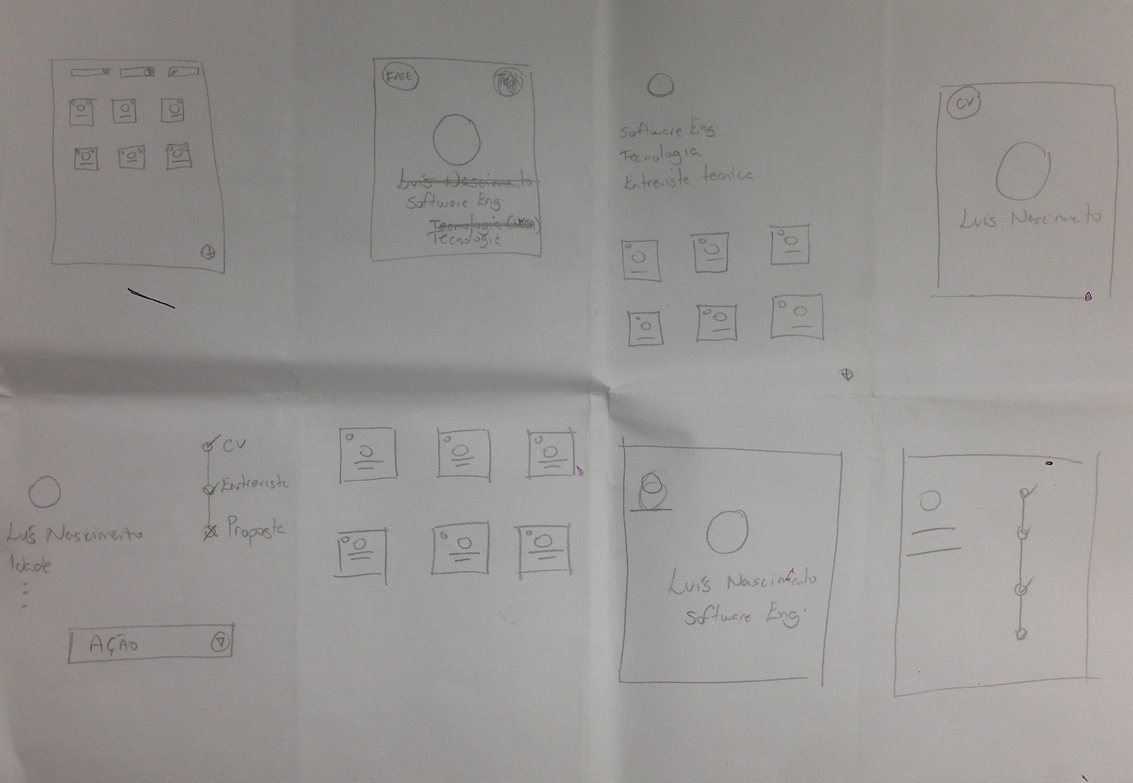
\includegraphics[width=\linewidth]{./04-figuras/06_biblioteca_componentes/crazy8.jpg}}
  \caption{Exemplo de artefato do \textit{Crazy Eights}}
  \fonte{Próprio autor}
  \label{fig:crazy8}
\end{figure}

A atividade de \textit{brainstorming} foi de fato um sucesso, gerando como saída vários artefatos e ideias que serviram de gatilho para o novo produto. Durante o processo, foi definido o primeiro entregável: a tela de \textit{login}.

Partiu-se, enfim, para a criação da biblioteca de componentes que seria utilizada como base para o desenvolvimento do novo sistema. Seguindo a ideia da Ryte \cite{ryteDesignSystem}, optou-se por dividir a biblioteca de componentes em dois grandes artefatos: um guia de design e um repositório com as implementações dos componentes.

A \autoref{fig:figma} ilustra a estrutura do guia de design produzido, já a \autoref{fig:sourceTree} apresenta a estrutura de arquivos do repositório que concentra as implementações dos componentes. Foi utilizado o Figma como ferramenta de criação do guia de design e o AngularJS \footnote{AngularJS é um framework JavaScript de código aberto, mantido pelo Google, que auxilia na execução de single-page applications.} como \textit{framework} base para implementação dos componentes. Percebe-se certa semelhança na forma como são organizadas as estruturas internas de cada artefato. Tal semelhança é reflexo do processo de co-criação do produto, onde os envolvidos no projeto tiveram participação ativa durante todo o processo, utilizando as mesmas terminologias para se referir aos componentes.

\begin{figure}
	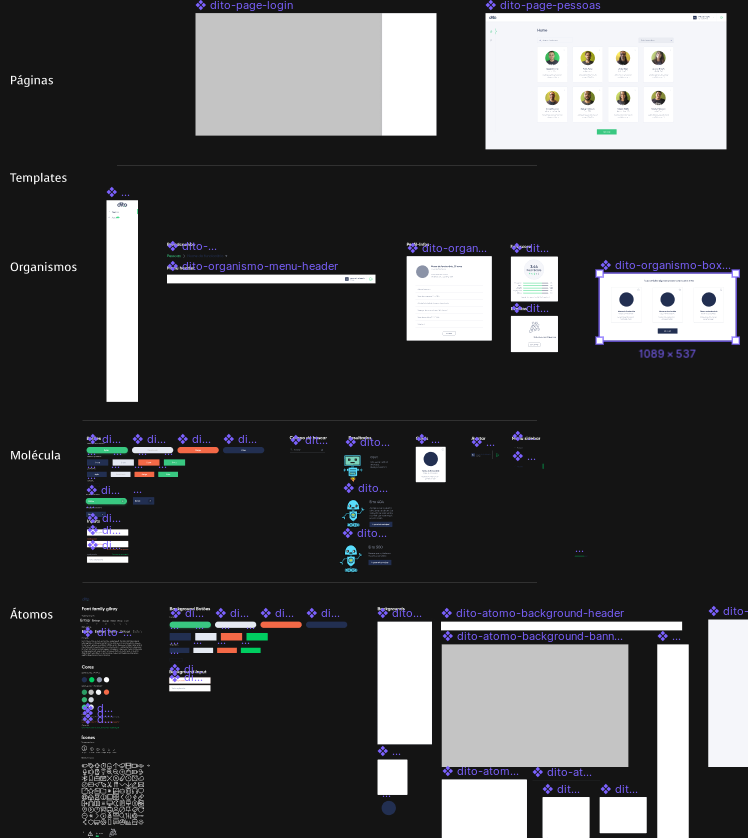
\includegraphics[width=\linewidth]{./04-figuras/06_biblioteca_componentes/styleguide-figma.png}
  \caption{Estrutura da biblioteca de componentes no Figma}
  \fonte{Próprio autor}
  \label{fig:figma}
\end{figure}

\begin{figure}
  \begin{center}
	  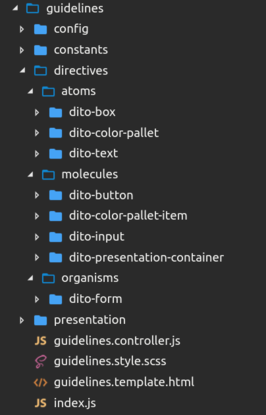
\includegraphics[]{./04-figuras/06_biblioteca_componentes/source-tree.png}
	\end{center}
  \caption{Árvore de diretórios da biblioteca de componentes}
  \fonte{Próprio autor}
  \label{fig:sourceTree}
\end{figure}

Seguindo a metodologia do \textit{Atomic Design} \cite{frostAtomicDesign}, os componentes do sistema foram construídos em uma estrutura \textit{bottom-up}, ou seja, do componente mais simples para o mais complexo. A seguir são apresentadas a anatomia de alguns dos componentes presentes no sistema.

\section{Átomos}

Os átomos são representações dos blocos básicos para a contrução de componentes mais complexos do sistema. O \autoref{table:atomsDitoFeras} apresenta o que foi entendido como átomo do sistema, além de descrever seu propósito.

\begin{quadro}
\centering
\begin{tabular}{|m{4cm}|m{10cm}|} \hline
	
	\multicolumn{1}{|c|}{\bfseries Nome} & \multicolumn{1}{c|}{\bfseries Descrição} \\\hline
	
	 \textit{dito-box} &  Representa um container de conteúdos. \\\hline
	 
	 \textit{dito-color-pallet} & Paleta de cores da aplicação. Padroniza o espectro de cores a ser utilizado ao longo do sistema. \\\hline
	 
	 \textit{dito-text} & Consolida os tipos de textos presentes no sistema. Deve abrangir semânticamente títulos, parágrafos, \textit{placeholders} e etc. Padroniza tamanhos de fonte, família da fonte, intensidade do texto e etc. \\\hline
    
\end{tabular}
\caption{Átomos do sistema \textit{DitoFeras}}
\fonte{Próprio autor}
\label{table:atomsDitoFeras}
\end{quadro}

Dos átomos listados, a paleta de cores é aquele que apresenta maior destaque, sendo de fundamental importância para garantir consistência na experiência do usuário ao utilizar o sistema. A \autoref{fig:colorPallet} apresenta a implementação desse componente.

\begin{figure}
  \begin{center}
	  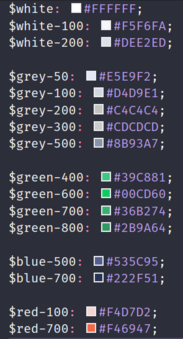
\includegraphics[]{./04-figuras/06_biblioteca_componentes/color-pallet.png}
	\end{center}
  \caption{Paleta de cores do sistema \textit{DitoFeras}}
  \fonte{Próprio autor}
  \label{fig:colorPallet}
\end{figure}

Percebe-se que a implementação do átomo da paleta de cores se restringe a um arquivo \textit{Sass} \footnote{\textit{Sass} é uma linguagem de folhas de estilo concebida inicialmente por Hampton Catlin e desenvolvida por Natalie Weizenbaum. Disponível em <https://sass-lang.com>} com definições de cores em variáveis. Não deve haver, ao longo das implementações dos outros componentes, nenhuma atribuição de cor que não utilize as variáveis definidas por este átomo.

\section{Moléculas}

As moléculas são conjuntos de átomos que, combinados, geram um valor mínimo para o usuário final. O \autoref{table:moleculesDitoFeras} apresenta o que foi entendido como molécula do sistema, além de descrever seu propósito.

\begin{quadro}
\centering
\begin{tabular}{|m{4cm}|m{10cm}|} \hline
	
	\multicolumn{1}{|c|}{\bfseries Nome} & \multicolumn{1}{c|}{\bfseries Descrição} \\\hline
	
	 \textit{dito-button} & Abstração dos possíveis botões do sistema. \\\hline
	 
	 \textit{dito-color-pallet-item} & Representa a forma apresentável de uma cor da paleta de cores. Inclui, além da cor em si, seu nome e sua representação em hexadecimal. \\\hline
	 
	 \textit{dito-input} & Abstração dos possíveis campos de entrada de texto do sistema. \\\hline
	 
	 \textit{dito-presentation-container} & Representa um container de componentes. Utilizado nas páginas de apresentação da biblioteca de componentes. \\\hline
    
\end{tabular}
\caption{Moléculas do sistema \textit{DitoFeras}}
\fonte{Próprio autor}
\label{table:moleculesDitoFeras}
\end{quadro}

Das moléculas listadas, o componente de botões é aquele que vale ser ressaltado. Diferentemente da simplicidade dos átomos, moléculas são componentes mais complexos e normalmente abstraem algum tipo de comportamento internamente. O \autoref{table:ditoButton} apresenta a anatomia do \textit{dito-button}, descrevendo sua interface de uso.

\begin{quadro}
\centering
\begin{tabular}{|m{4cm}|m{3cm}|m{7cm}|} \hline
	
	\multicolumn{1}{|c|}{\bfseries Atributo} & \multicolumn{1}{c|}{\bfseries Tipo} & \multicolumn{1}{c|}{\bfseries Descrição} \\\hline
	
	 \textit{type} & \textit{string} & Define o tipo do botão. São reconhecidos dois tipos: padrão e envio (\textit{submit}). Caso não informado, assume-se o valor padrão. \\\hline
	 \textit{onClick} & \textit{function} & Função que será executada após algum evento de clique por parte do usuário. \\\hline
	 \textit{isDisabled} & \textit{boolean} & Informa se o botão está em um estado desabilitado, ou não. Quando desabilitado, ações de clique, por parte do usuário, são ignoradas. \\\hline
    
\end{tabular}
\caption{Interface de uso do componente \textit{dito-button}}
\fonte{Próprio autor}
\label{table:ditoButton}
\end{quadro}

Pode-se perceber que o componente \textit{dito-button} possui um mecanismo de estado associado. Dessa forma, o comportamento do componente depende diretamente do estado atual do mesmo. A \autoref{fig:buttons} ilustra o componente nos seus seis diferentes tipos de estado.

\begin{figure}
  \begin{center}
	  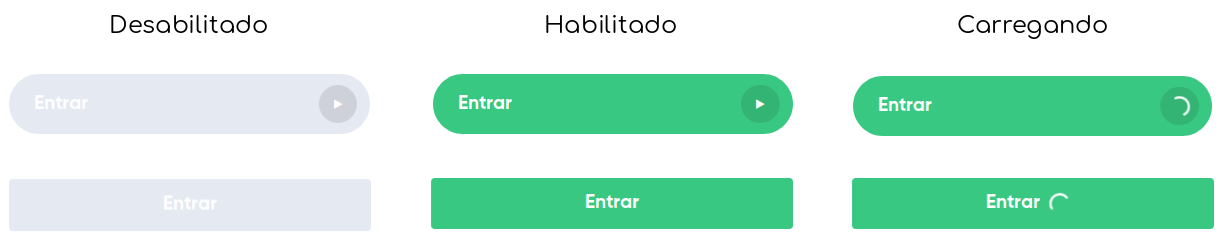
\includegraphics[width=\linewidth]{./04-figuras/06_biblioteca_componentes/buttons.png}
	\end{center}
  \caption{Estados de um botão do sistema \textit{DitoFeras}}
  \fonte{Próprio autor}
  \label{fig:buttons}
\end{figure}

\section{Organismos}

Organismos são grupos de moléculas que, juntas, formam uma seção relativamente complexa e distinta da interface de usuário. Até o momento em que o presente trabalho foi escrito, o único organismo implementado no sistema foi o \textit{dito-form}, que encapsula lógicas de validação de formulários de envio de dados para o servidor. A \autoref{fig:forms} ilustra um formulário de \textit{login} em três diferentes estados.

\begin{figure}
  \begin{center}
	  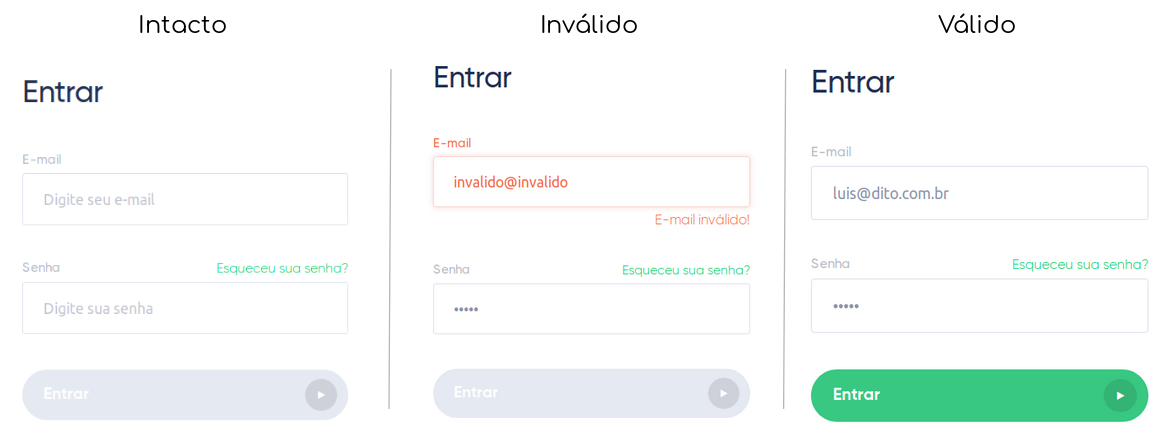
\includegraphics[width=\linewidth]{./04-figuras/06_biblioteca_componentes/forms.png}
	\end{center}
  \caption{Estados de um formulário de \textit{login} do sistema \textit{DitoFeras}}
  \fonte{Próprio autor}
  \label{fig:forms}
\end{figure}

Por estratégia do autor, não foram implementadas as abstrações de templates proposta pela metodologia do \textit{atomic design}, uma vez que a reusabilidade de páginas seria mínima em um estágio inicial de projeto.

No capítulo seguinte serão apresentadas as páginas implementadas do sistema que utilizaram a biblioteca de componentes ilustrada neste capítulo como blocos básicos de sua construção. % Biblioteca de componentes
% -----------------------------------------------------------------------------
% Páginas Web
% -----------------------------------------------------------------------------

\chapter{Desenvolvimento de Páginas Web}
\label{chap:devWeb}

O sétimo capítulo do presente trabalho tem como objetivo a implementação de páginas Web utilizando a biblioteca de componentes previamente desenvolvida. As seções a seguir detalharão o processo de criação das interfaces de usuários desenvolvidas nesta fase: telas de listagem de componentes e tela de \textit{login}.

\section{Telas de listagem de componentes}
\label{sec:listaComponentes}

Como forma de garantir um ponto focal para a documentação da biblioteca de componentes, as primeiras páginas Web implementadas foram aquelas que apresentavam os componentes criados. A \autoref{fig:listComponentsButton} apresenta uma das páginas de apresentação de componente: a página do componente \textit{dito-button}.

Desejava-se que todas as páginas criadas fossem baseadas na biblioteca de componentes, entretanto tanto o cabeçalho quanto a seção de navegação da página não foram definidos por ela em sua primeira versão. Faz-se necessária uma refatoração do código-fonte, no futuro, para abstrair tais elementos para componentes da biblioteca.

\begin{figure}
  \begin{center}
	  \frame{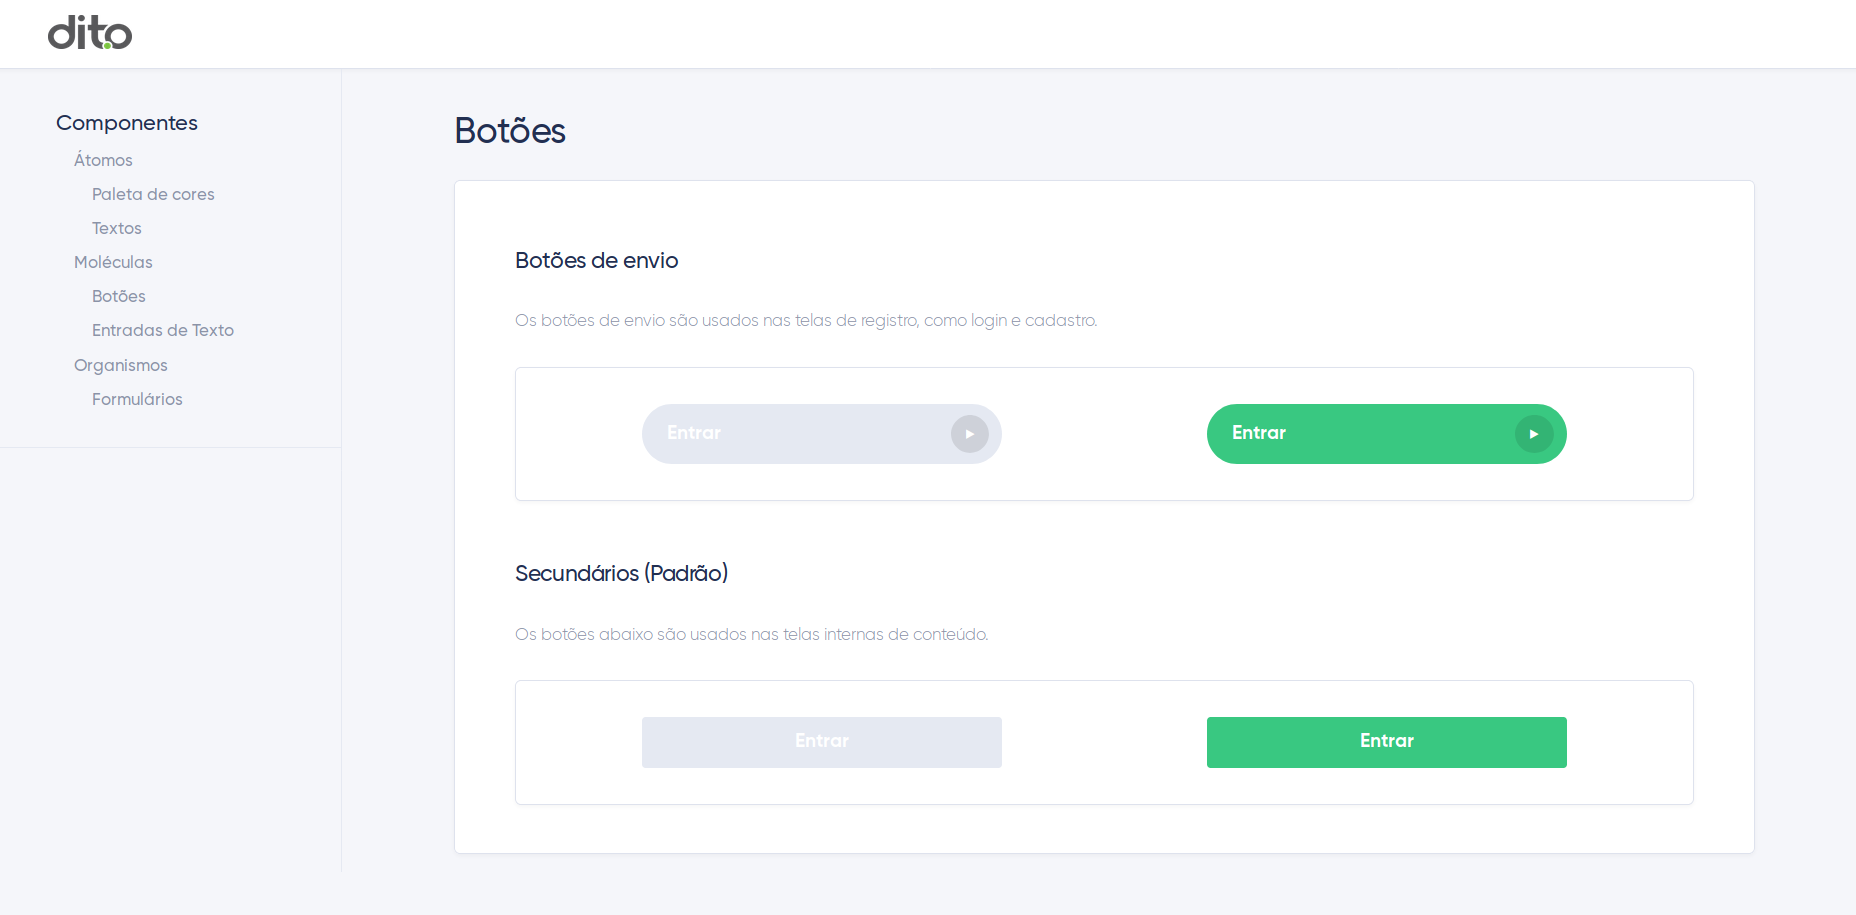
\includegraphics[width=\linewidth]{./04-figuras/07_paginas_web/lista-componentes.png}}
	\end{center}
  \caption{Página de apresentação do componente \textit{dito-button}}
  \fonte{Próprio autor}
  \label{fig:listComponentsButton}
\end{figure}

\section{Tela de \textit{login}}
\label{sec:telaLogin}

A primeira página implementada para o projeto \textit{DitoFeras} foi a página de \textit{login}. A \autoref{fig:loginPage} ilustra o resultado final de sua implementação.

\begin{figure}
  \begin{center}
	  \frame{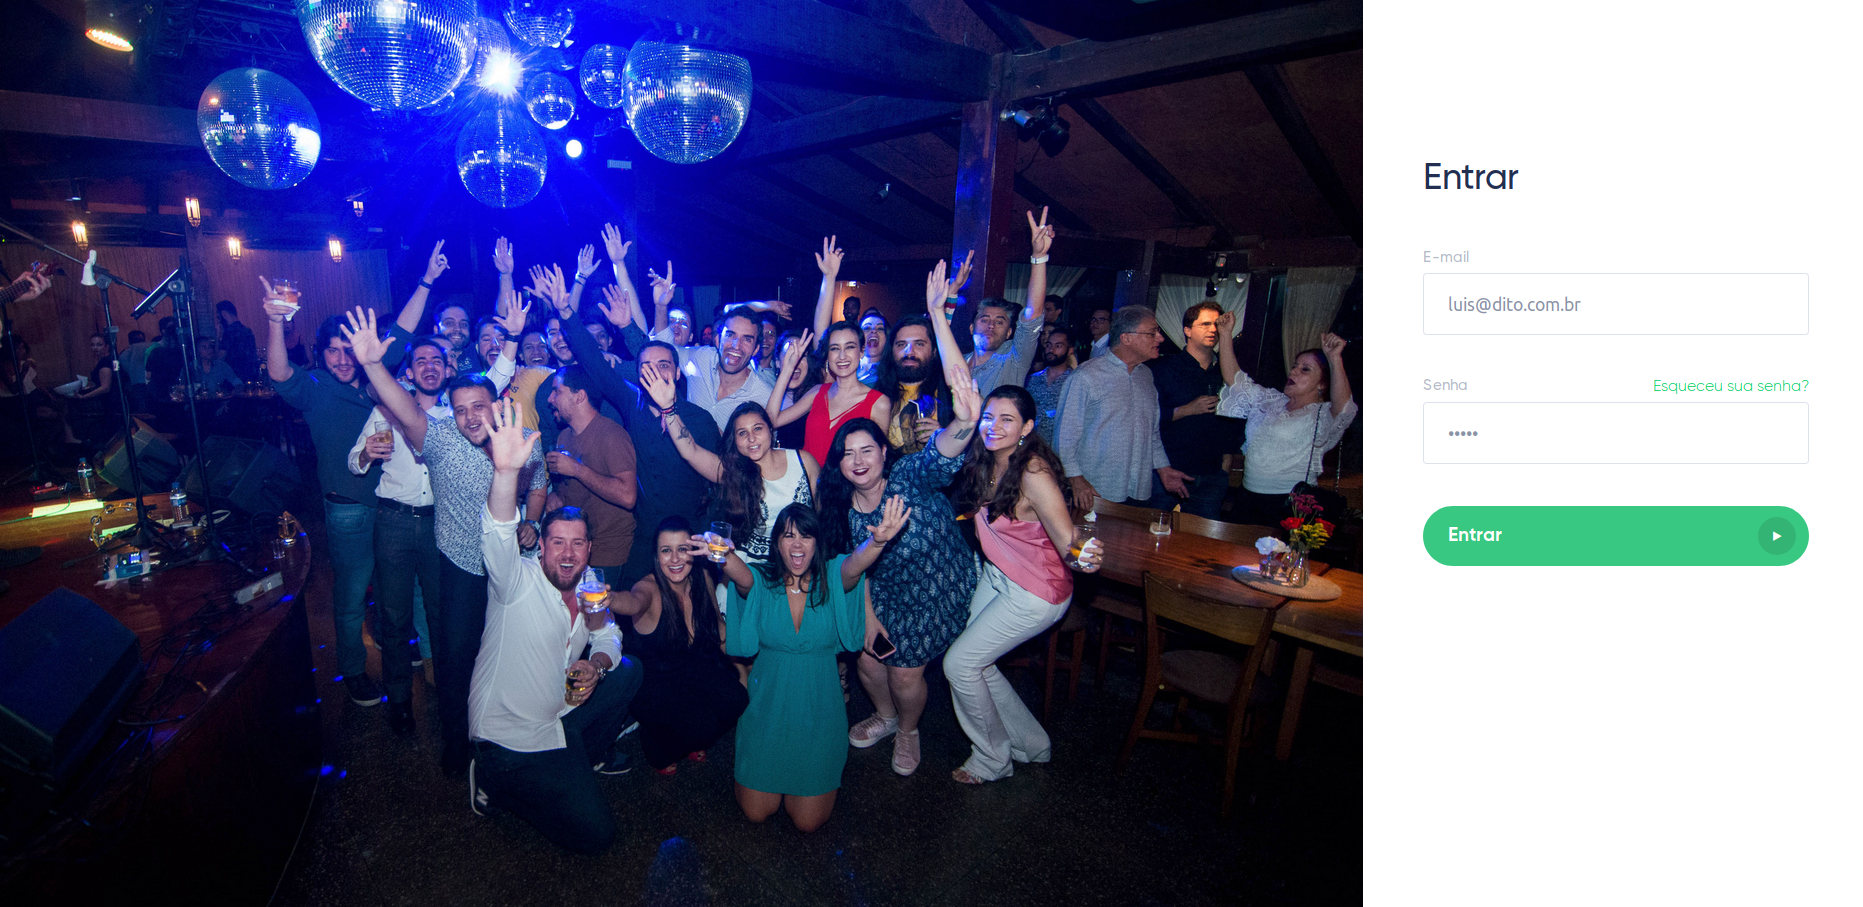
\includegraphics[width=\linewidth]{./04-figuras/07_paginas_web/login.png}}
	\end{center}
  \caption{Página de \textit{login} do sistema \textit{DitoFeras}}
  \fonte{Próprio autor}
  \label{fig:loginPage}
\end{figure}

Diferentemente das páginas de listagem de componentes, esta foi construida utilizando única e exclusivamente os componentes da biblioteca. A \autoref{fig:loginCode} apresenta todo o código-fonte necessário para a construção da página de \textit{login}. Fica evidente o quão simples é o desenvolvimento de novas interfaces de usuários baseadas em componentes previamente implementadas. Muito do comportamento da página acaba já sendo implementado pelos componentes envolvidos, restando assim apenas o esforço de posiciona-los adequadamente ao longo da interface.

\begin{figure}
  \begin{center}
	  \frame{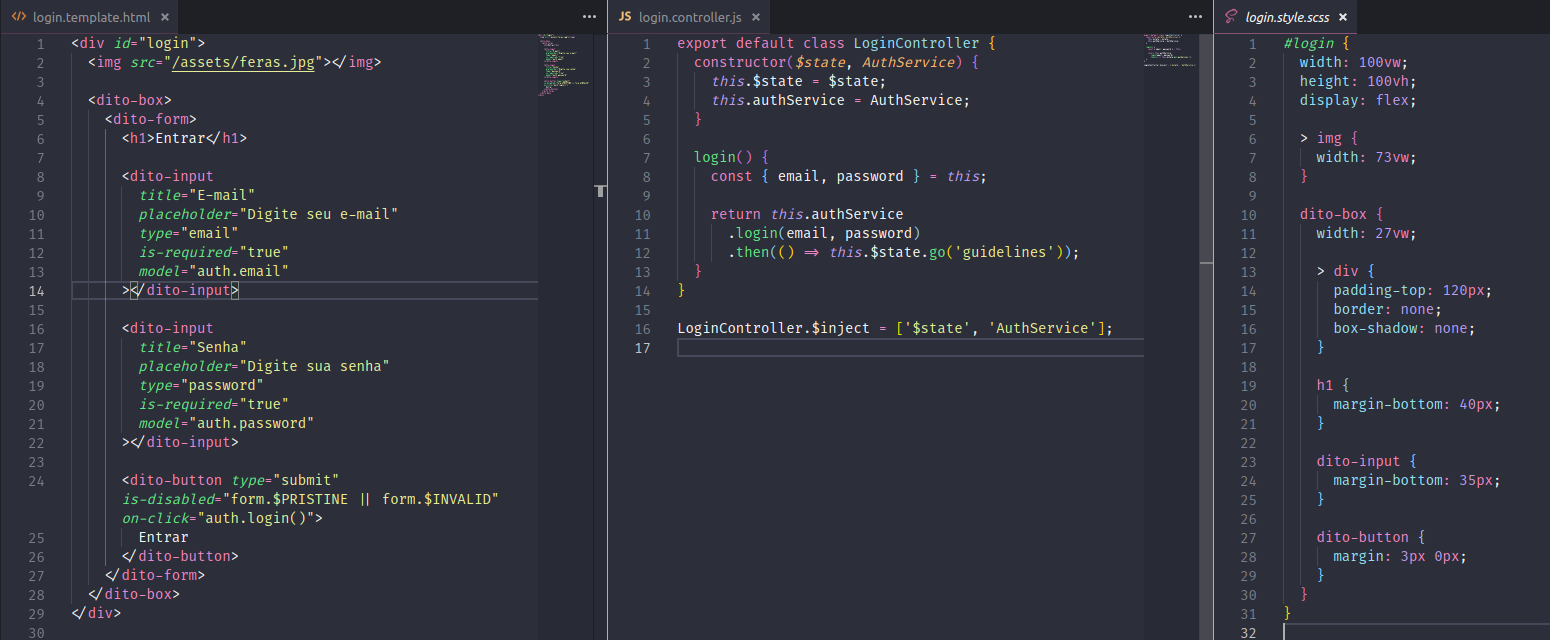
\includegraphics[width=\linewidth]{./04-figuras/07_paginas_web/login-code.png}}
	\end{center}
  \caption{Código-fonte da página de \textit{login} do sistema \textit{DitoFeras}}
  \fonte{Próprio autor}
  \label{fig:loginCode}
\end{figure}

No capítulo seguinte é discutida, detalhadamente, a avaliação dos resultados obtidos através do presente trabalho.
            % Páginas Web
% -----------------------------------------------------------------------------
% Resultados
% -----------------------------------------------------------------------------

\chapter{Avaliação de Resultados}
\label{chap:resultados}

O presente capítulo é destinado à discussão dos resultados obtidos durante o desenvolvimento deste trabalho. A discussão é dividida em 2 momentos: resultados das entrevistas com \textit{stakeholders} e resultados do protótipo de biblioteca de componentes.

\section{Entrevistas com \textit{stakeholders}}
\label{sec:resEntrevistas}

No capítulo 5 deste trabalho, foi apresentada detalhadamente uma visão consolidada da percepção técnica de designers e desenvolvedores \textit{frontend} em relação à plataforma da empresa avaliada no experimento. Muitas das dores e frustrações compartilhadas por empresas que adotaram a metodologia do \textit{design system} como meio de transformação dos processos de design do seu produto, e que foram apresentadas no capítulo 3, também puderam ser percebidas pelos entrevistados.

Tomando como base as experiências compartilhadas pelos entrevistados e o \autoref{table:uxMaturity}, entende-se que a empresa avaliada encontra-se no terceiro estágio de maturidade em experiência do usuário: Embrionária. Tal classificação é justificada pelo fato de que, apesar de já existirem profissionais especializados que se preocupam com a experiência do usuário, atividades de planejamento e metrificação de valores de UX ainda não acontecem com consistência. Também não existe nenhum profissional focado em definir e disseminar diretrizes de design e UX a nível organizacional. Dessa forma, fica evidente que ainda existe um longo caminho a ser percorrido pela organização no que se diz respeito à evolução de sua maturidade de UX, e para que isso ocorra, o comprometimento de toda a organização tem vital importância.

Como forma de se medir quantitativamente o nível de satisfação dos entrevistados para com o produto da empresa, foi realizada uma simples pesquisa com os envolvidos. A pesquisa, apresentada no Apêndice C deste projeto, indagava, em uma escala de 1 a 10, qual o nível de satisfação do entrevistado em relação a 3 aspectos chave do produto da empresa: capacidade de escalabilidade, capacidade de reusabilidade e velocidade de desenvolvimento. A \autoref{fig:productMetrics} apresenta os resultados obtidos pela pesquisa.

\begin{figure}
  \begin{center}
	  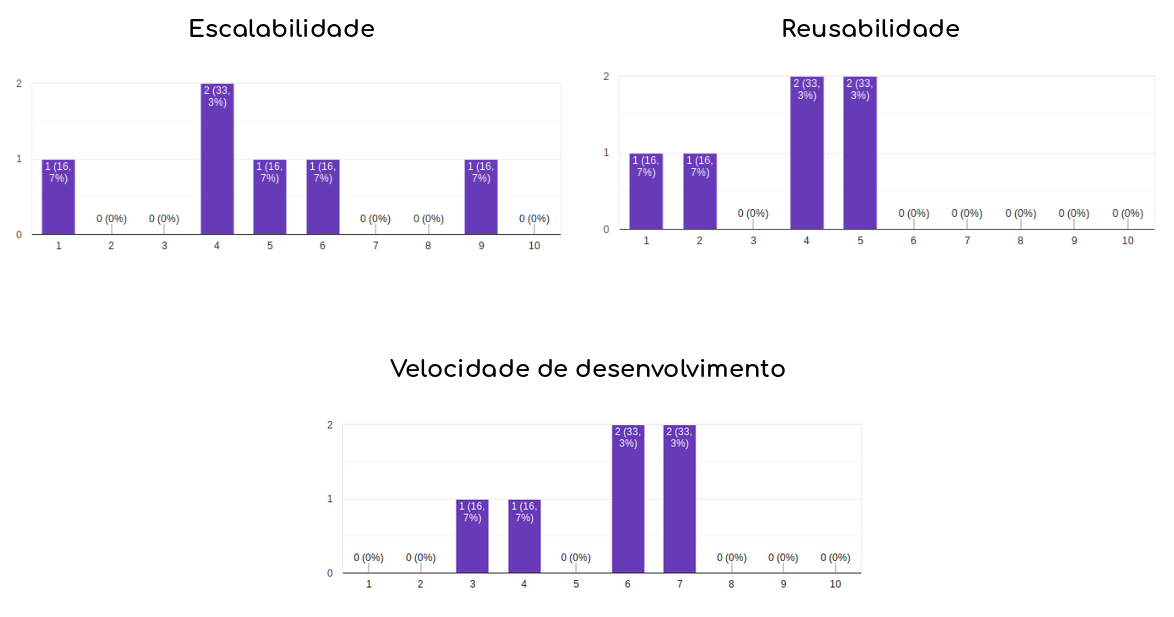
\includegraphics[width=\linewidth]{./04-figuras/08_avaliacao_resultados/product-metrics.png}
	\end{center}
  \caption{Nível de satisfação da arquitetura do produto da Dito}
  \fonte{Próprio autor}
  \label{fig:productMetrics}
\end{figure}

Para traduzir os resultados da pesquisa em um número único que reflita a atual realidade da arquitetura do produto da empresa, foi utilizada a metodologia do NPS. Em termos gerais, o \textit{Net Promoter Score} (NPS) trata-se de uma pesquisa de satisfação criada em 2003 por Fred Reichheld que, por ser simples e de fácil aplicação, acabou sendo adotada por muitas empresas, tornando-se um método universal de avaliação da satisfação de clientes \cite{nps}. Para a metodologia, as respostas da pesquisa são classificadas em 3 grupos:

\begin{itemize}
  \item Promotores: Nota 9 ou 10
  \item Neutros: Nota 7 ou 8
  \item Detratores: Notas de 1 a 6
\end{itemize}

Para o calculo do NPS, utiliza-se a seguinte fórmula:
\begin{center}
  \textbf{(Promotores - Detratores) / total de respondentes}.    
\end{center}{}

A metodologia ainda classifica os possíveis resultados do cálculo do NPS em 4 grupos:

\begin{itemize}
  \item Zona de excelência: 75\% -- 100\%
  \item Zona de qualidade: 50\% -- 74\%
  \item Zona de aperfeiçoamento: 0\% -- 49\%
  \item Zona crítica: -100\% -- -1\%
\end{itemize}

A \autoref{table:productNPS} apresenta o cálculo do NPS para as 3 diretrizes consultadas. A partir dela, conclui-se que a arquitetura do produto da empresa encontra-se em uma zona crítica, implicando que medidas devem ser tomadas o quanto antes para que a atual realidade seja revertida.

\begin{table}
  \centering
  \begin{tabular}{|m{6cm}|m{2cm}|} \hline
    
    \multicolumn{1}{|c|}{\bfseries Diretriz} & \multicolumn{1}{c|}{\bfseries NPS} \\\hline
    
    Escalabilidade & -66,67\% \\\hline
    Reusabilidade & -100\% \\\hline
    Velocidade de desenvolvimento & -66,67\% \\\hline
      
  \end{tabular}
  \caption{NPS da arquitetura do produto da Dito}
  \fonte{Próprio autor}
  \label{table:productNPS}
\end{table}


\section{Protótipo da biblioteca de componentes}

Para avaliar o valor do protótipo de biblioteca de componentes desenvolvido, foram levantadas 2 métricas base para a análise: nível de consistência das interfaces e quantidade de linhas de código-fonte. As subseções a seguir detalham cada uma das métricas, levando em consideração o atual cenário do produto da Dito e o protótipo implementado.

\subsection{Consistência nas interfaces de usuário}

Para medir a consistência em interfaces de usuário, foi realizada uma contagem do número de cores, cores de fundo, famílias de fonte e tamanhos de fonte distintos presentes nos dois objetos de estudo. A \autoref{table:interfaceConsistence}, consolida tais números.

\begin{table}
  \centering
  \begin{tabular}{|m{3cm}|m{1cm}|m{1cm}|m{1cm}|m{1cm}|} \hline
    
    \multicolumn{1}{|c|}{\bfseries Sistema} & \multicolumn{1}{c|}{\bfseries Cores} & \multicolumn{1}{c|}{\bfseries Cores de fundo} & \multicolumn{1}{c|}{\bfseries Famílias de fonte} & \multicolumn{1}{c|}{\bfseries Tamanhos de fonte} \\\hline
    
    Principal produto da Dito & 63 & 88 & 4 & 41 \\\hline
    \textit{Dito Feras} & 12 & 7 & 1 & 7 \\\hline
      
  \end{tabular}
  \caption{Consistência de interfaces de usuário}
  \fonte{Próprio autor}
  \label{table:interfaceConsistence}
\end{table}

Obviamente, comparar friamente os números dos dois sistemas não seria adequado, uma vez que o produto da empresa avaliada é muito maior e mais complexo do que o protótipo construído por este trabalho. Entretanto, contanto que a biblioteca de componentes continue evoluindo de maneira saudável, espera-se que as inconsistências evidenciadas no principal produto da Dito não se manifestem em sistemas construídos a partir de tal biblioteca.

\subsection{Quantidade de linhas de código-fonte}

Para medir fatores como velocidade de desenvolvimento, capacidade de reusabilidade e capacidade de escalabilidade, optou-se por utilizar a métrica de quantidade de linhas de código-fonte necessárias para a implementação de uma dada funcionalidade. Nesse contexto, a \autoref{table:lineCountDitoFeras} apresenta a quantidade de linhas de código-fonte utilizadas para construir artefatos do sistema \textit{DitoFeras}, já a \autoref{table:lineCountDito} faz a mesma análise levando em consideração 4 interfaces de usuários recentemente implementadas no produto da Dito.

\begin{table}
\centering
\begin{tabular}{|m{10cm}|m{1cm}|m{1cm}|m{1cm}|m{1cm}|} \hline
	
	\multicolumn{1}{|c|}{\bfseries Artefato} & \multicolumn{1}{c|}{\bfseries HTML} & \multicolumn{1}{c|}{\bfseries CSS} & \multicolumn{1}{c|}{\bfseries Javascript} \\\hline
	
	 Componente \textit{dito-box} & 0 & 9 & 10 \\\hline
	 Componente \textit{dito-color-pallet} & 0 & 20 & 0 \\\hline
	 Componente \textit{dito-text} & 0 & 64 & 0 \\\hline
	 
	 Componente \textit{dito-button} & 11 & 188 & 29 \\\hline
	 Componente \textit{dito-color-pallet-item} & 9 & 21 & 14 \\\hline
	 Componente \textit{dito-input} & 19 & 98 & 102 \\\hline
	 Componente \textit{dito-presentation-container} & 4 & 21 & 15 \\\hline
	 
	 Componente \textit{dito-form} & 0 & 0 & 34 \\\hline
	 
	 Tela de \textit{login} & 29 & 31 & 16 \\\hline
	 Tela de apresentação do componente \textit{dito-color-pallet} & 14 & 9 & 20 \\\hline
	 Tela de apresentação do componente \textit{dito-text} & 10 & 0 & 0 \\\hline
	 Tela de apresentação do componente \textit{dito-button} & 29 & 9 & 10 \\\hline
	 Tela de apresentação do componente \textit{dito-input} & 48 & 9 & 22 \\\hline
	 Tela de apresentação do componente \textit{dito-form} & 25 & 11 & 0 \\\hline
    
\end{tabular}
\caption{Quantidade de linhas de código-fonte por artefato do projeto \textit{DitoFeras}}
\fonte{Próprio autor}
\label{table:lineCountDitoFeras}
\end{table}


\begin{table}
\centering
\begin{tabular}{|m{3cm}|m{1cm}|m{1cm}|m{1cm}|m{1cm}|} \hline
	
	\multicolumn{1}{|c|}{\bfseries Artefato} & \multicolumn{1}{c|}{\bfseries HTML} & \multicolumn{1}{c|}{\bfseries CSS} & \multicolumn{1}{c|}{\bfseries Javascript} \\\hline
	 Tela 1 & 467 & 1046 & 203 \\\hline
	 Tela 2 & 98 & 257 & 258 \\\hline
	 Tela 3 & 348 & 603 & 398  \\\hline
	 Tela 4 & 837 & 1199 & 608 \\\hline
    
\end{tabular}
\caption{Quantidade de linhas de código-fonte por artefato do produto da Dito}
\fonte{Próprio autor}
\label{table:lineCountDito}
\end{table}

Guardadas as devidas proporções, percebe-se que o esforço para se construir interfaces de usuários baseadas em componentes previamente implementados é consideravelmente mais baixo. Existe um esforço inicial para se construir os componentes base das páginas, porém, uma vez implementados, o desenvolvimento de novas interfaces de usuário demonstra-se ser uma tarefa relativamente simples.

É importante mencionar, porém, que apesar de haver bastante duplicidade de código entre as soluções, as 4 interfaces selecionadas do produto da Dito para o comparativo são consideravelmente mais complexas do aquelas produzidas no protótipo. Por esse motivo, a comparação entre os números dos dois sistemas não deve acontecer de maneira literal.

Dada a simplicidade percebida no desenvolvimento de páginas baseadas em componentes, entendeu-se que o protótipo construído cumpriu o seu propósito. O valor de uma biblioteca de componentes, que no futuro poderia ser evoluída para um \textit{design system} completo e robusto, foi entendido pelos \textit{stakeholders} do projeto.

Ressalta-se, entretanto, que a escolha da tecnologia utilizada para a construção do protótipo foi falha. A empresa avaliada no experimento tinha pretenções de evoluir sua arquitetura \textit{frontend}, alterando o \textit{framework} base de suas implementações. Como a biblioteca de componentes foi construida utilizando um \textit{framework} diferente, seria inviável aproveitar o trabalho realizado na construção do protótipo em uma futura biblioteca de componentes oficial da organização.

Sabe-se que o ecossistema de tecnologia está em constante evolução. Novas tecnologias surgem a cada dia e, consequentemente, as tecnologias de ponta de hoje acabarão se tornando defasadas no futuro. Nesse contexto, entendeu-se a criação de um sistema tão importante como uma biblioteca de componentes baseado em um \textit{framework} específico não é uma decisão sustentável a longo prazo. A utilização de tecnologias como \textit{Web Components} talvez seja uma decisão mais sábia, uma vez que esta é baseada em padrões universais da Web.

Como consequência do presente trabalho, foi criado um grupo de estudos na empresa avaliada no experimento. O objetivo principal do grupo é disseminar conhecimentos a respeito dos propósitos e valores de um \textit{design system}. Foi realizada, ainda, uma atividade de descontrução de um dos mais recentes produtos da empresa, com o intuito de idealizar o esqueleto de uma biblioteca de componentes que siga os princípios do \textit{atomic design}.

Finalmente, conclui-se que um \textit{design system} é uma importante ferramenta para a diminuição da complexidade social de uma organização, promovendo melhorias na comunicação entre os colaboradores desde os momentos iniciais de sua implementação. Além disso, também se provou fundamental para a alavancagem da capacidade de escalabilidade, reusabilidade e velocidade de desenvolvimento de produtos baseados em software.
             % Resultados
% -----------------------------------------------------------------------------
% Conclusão
% -----------------------------------------------------------------------------

\chapter{Conclusão}
\label{chap:conclusao}

Este trabalho realizou um estudo a respeito da viabilidade de implementação de um \textit{design system} em uma empresa de tecnologia de médio porte. A metodologia adotada durante a avaliação consistiu em uma fase de entrevistas, onde desejava-se entender se os colaboradores da organização ansiavam por uma ferramenta de tal natureza, além de uma fase de implementação, onde foi desenvolvido um protótipo do sistema desejado.

Os resultados obtidos durante a etapa de entrevistas estão completamente alinhados com o que foi observado nos estudos de trabalhos relacionados. Problemas como inconsistências de usabilidade do produto, lento ciclo de desenvolvimento e a falta de diretrizes claras e objetivas que guiam a tomada de decisões de design, são fatores comuns que prejudicam a capacidade de escalabilidade dos produtos a longo prazo. Além disso, foi constatado que, conforme uma organização cresce em termos de número de funcionários, mais difícil se torna a gestão de comunicação e do conhecimento interno. Nesse contexto, um \textit{design system} cumpre o papel fundamental de centralização do conhecimento e diminuição da complexidade social de uma empresa.

Durante a fase de implementação, por sua vez, ficou clara a maneira como a existência de uma biblioteca de componentes bem estrutura impacta positivamente a velocidade de desenvolvimento e o nível de consistência de um produto. Ressalta-se, entretanto, a preocupação de não se criar dependência alguma entre a biblioteca de componentes e \textit{frameworks} ou tecnologias específicas, uma vez que isso contribui para o fenômeno de defasamento da ferramenta.

Também foi percebido que a criação de um \textit{design system} completo não é uma tarefa fácil de ser realizada. Para tanto, faz-se necessário o envolvimento e participação de profissionais das mais diversas áreas de atuação, uma vez que a ferramenta se propõe a atender às necessidades da organização como um todo. O maior desafio, portanto, seria manter a ferramenta constantemente atualizada, garantindo que a mesma não caia em desuso.

Finalmente, como sugestão de trabalho futuro é proposta a criação de uma nova biblioteca de componentes, dessa vez utilizando a tecnologia conhecida como \textit{Web Componentes}, baseada em um dos produtos mais recentes da empresa avaliada no experimento do presente trabalho. Tal produto já possui uma identidade visual mais moderna e bem padronizada. Em sequência, as próximas atividades a serem executadas seriam a definição dos artefatos de Tom de Voz e Princípios de Design, concluindo assim um \textit{design system} completo que transformará a maneira que a plataforma da empresa é gerenciada.
              % Conclusão

% Insere os elementos pós-textuais
\postextual
% -----------------------------------------------------------------------------
% Referências
% -----------------------------------------------------------------------------

% Carrega o arquivo "referencias.bib" com as referências do trabalho
\bibliography{./referencias}{}

% Define o estilo ABNT para formatar a lista de referências
\bibliographystyle{abntex2-alf}

% -----------------------------------------------------------------------------
% Não é necessário editar este arquivo.
% -----------------------------------------------------------------------------
        % Referências
% -----------------------------------------------------------------------------
% Anexos
% -----------------------------------------------------------------------------

\begin{anexosenv}
\partanexos

% -----------------------------------------------------------------------------
% Anexo A: Estrutura de entrevista com designer
% -----------------------------------------------------------------------------

\chapter{Estrutura de entrevista com designer}
\label{chap:anexoA}

\begin{itemize}
  \item Conte um pouco sobre seu \textit{background} na empresa.
  \item Contextualize, brevemente, a maneira como os processos de design são adotados na empresa, atualmente.
  \item Quais as maiores dificuldades e frustrações que você encontra no seu trabalho, como consequência dos processos atuais de design?
  \item Como são tomadas decisões de design na empresa? E no seu time? Quem são as pessoas envolvidas?
  \item Como você classifica a velocidade de desenvolvimento de novas interfaces de usuários atualmente? Por que?
  \item Você acredita que um \textit{design system} poderia ser uma opção plausível para alavancar a capacidade de escalabilidade do produto da empresa?
  \item Mais alguma idéia, dúvida ou comentário a respeito de \textit{design systems}?
\end{itemize}

% -----------------------------------------------------------------------------
% Anexo B: Estrutura de entrevista com desenvolvedor
% -----------------------------------------------------------------------------

\chapter{Estrutura de entrevista com desenvolvedor}
\label{chap:anexoB}

\begin{itemize}
  \item Conte um pouco sobre seu \textit{background} na empresa.
  \item Contextualize, brevemente, a maneira como os processos de desenvolvimento \textit{frontend} são adotados na empresa, atualmente.
  \item Quais as maiores dificuldades e frustrações que você encontra na plataforma durante o desenvolvimento de suas atividades?
  \item Você participa das decisões de design das suas entregas? Faz(ria) sentido para você participar? Por que?
  \item Como você classifica a velocidade de desenvolvimento de novas interfaces de usuários atualmente? Por que?
  \item Como você classifica o esforço para se realizar manutenção em interfaces de usuário já existentes na plataforma atualmente?
  \item De modo geral, como você classifica a atual arquitetura \textit{frontend} da plataforma a nível de escalabilidade e reusabilidade?
  \item Você já ouviu falar no termo \textit{design system}? Se sim, acredita que poderia ser uma abordagem plausível para impulsinar a capacidade de escalabilidade do produto da empresa?
  \item Mais alguma idéia, dúvida ou comentário a respeito de \textit{design systems}?
\end{itemize}

% -----------------------------------------------------------------------------
% Anexo C: Pesquisa de satisfação da arquitetura do produto da Dito
% -----------------------------------------------------------------------------

\chapter{Pesquisa de satisfação da arquitetura do produto da Dito}
\label{chap:anexoC}

\begin{itemize}
	\item Em uma escala de 1 a 10, sendo 1 extremamente lenta e 10 extremamente rápida, como você classificaria a velocidade de desenvolvimento de novas interfaces de usuário na plataforma da Dito?
	\item Em uma escala de 1 a 10, sendo 1 terrível e 10 excelente, como você classificaria o poder de reusabilidade de componentes na plataforma da Dito?
	\item Em uma escala de 1 a 10, sendo 1 terrível e 10 excelente, como você classificaria a capacidade de escalabilidade da plataforma da Dito?
\end{itemize}

\end{anexosenv}
             % Anexos
% -----------------------------------------------------------------------------
% Índice Remissivo
% -----------------------------------------------------------------------------

% -----------------------------------------------------------------------------
% Este comando gera automaticamente o índice remissivo para os termos definidos
% no corpo do documento.
% -----------------------------------------------------------------------------

\printindex

% -----------------------------------------------------------------------------
% Não é necessário editar este arquivo.
% -----------------------------------------------------------------------------
   % Índice Remissivo

\end{document}
